% =========================================================
% Introduction to Algebraic Structures
% Notes Router
% =========================================================

\begin{topicbox}[Where You Are in the Journey]
\begin{center}
\small
Propositional Logic
$\;\to\;$ Predicate Calculus
$\;\to\;$ Sets \& Functions
$\;\to\;$ Proof Techniques
$\;\to\;$ Real Analysis
$\;\to\;$ \textbf{Intro to Algebraic Structures}
$\;\to\;$ Linear Algebra
$\;\to\;$ Topology
$\;\to\;$ $\cdots$
\end{center}

\medskip
\noindent
This chapter fixes the vocabulary of algebraic structure first, then builds
the standard one-law and two-law structure tower by adding one axiom at a
time.
\end{topicbox}

\section{What Is a Mathematical Structure?}

% =========================================================
% Chapter 1 Locked Refactor: Part A
% =========================================================

\subsection{Algebraic Structures}
\label{sec:algebraic-structures}

\begin{remark*}[Geometric picture]
Before any specific algebra, fix what kind of thing we are studying: a set
of elements together with stipulated ways to combine them, compare them, and
name some of them. The axioms say which stipulations we keep. A group, a
ring, and a field are the same general idea with different stipulations.
\end{remark*}

\begin{definitionbox}{Definition (Algebraic Structure)}
\begin{definition}[Algebraic Structure]
\label{def:algebraic-structure}
An \textbf{algebraic structure} of signature $\mathcal L$ is a pair
\[
  \mathcal A=(A,I)
\]
where $A$ is a nonempty carrier set and $I$ interprets each symbol of
$\mathcal L$ on $A$: each $n$-ary function symbol as an operation
$A^n\to A$, each $n$-ary relation symbol as a subset of $A^n$, and each
constant symbol as an element of $A$. The structure is algebraic when
$\mathcal L$ has no relation symbols beyond equality.
\end{definition}
\end{definitionbox}

\begin{remark*}[Standard quantified statement]
\[
\operatorname{AlgStructure}_{\mathcal L}(\mathcal A)
\Longleftrightarrow
\mathcal A=(A,I),\ A\neq\varnothing,\ \text{and } I
\text{ interprets every symbol of }\mathcal L\text{ on }A.
\]
\end{remark*}

\begin{remark*}[Interpretation]
The signature is the type; the structure is the instance. ``Group'' is a
signature with a binary operation, an identity constant, and an inverse
operation; a particular group interprets these on a carrier.
\end{remark*}

\begin{remark*}[Bourbaki anchor]
Species of structure, \textit{Theory of Sets}, Chapter IV, Section 1.
\end{remark*}

\begin{dependencies}
\begin{itemize}
  \item \hyperref[def:carrier-set]{Carrier Set}
  \item \hyperref[def:signature]{First-Order Signature}
\end{itemize}
\end{dependencies}

\begin{definitionbox}{Definition (First-Order Signature)}
\begin{definition}[First-Order Signature]
\label{def:signature}
A \textbf{first-order signature}
\[
  \mathcal L=(\operatorname{Const}_{\mathcal L},
  \operatorname{Func}_{\mathcal L},
  \operatorname{Rel}_{\mathcal L},\operatorname{arity})
\]
lists constant symbols, function symbols, and relation symbols, with each
function or relation symbol carrying a declared arity.
\end{definition}
\end{definitionbox}

\begin{dependencies}
\begin{itemize}
  \item \hyperref[def:nullary]{Nullary Operation}
  \item \hyperref[def:unary]{Unary Operation}
  \item \hyperref[def:binop]{Binary Operation}
\end{itemize}
\end{dependencies}

\begin{definitionbox}{Definition ($\mathcal L$-Structure)}
\begin{definition}[$\mathcal L$-Structure]
\label{def:l-structure}
Given a signature $\mathcal L$, an \textbf{$\mathcal L$-structure} is a
nonempty carrier set $A$ together with an interpretation of every symbol of
$\mathcal L$ on $A$.
\end{definition}
\end{definitionbox}

\begin{dependencies}
\begin{itemize}
  \item \hyperref[def:signature]{First-Order Signature}
  \item \hyperref[def:carrier-set]{Carrier Set}
\end{itemize}
\end{dependencies}

% =========================================================
% Chapter 1 Locked Refactor: Part B
% =========================================================

\subsection{Laws of Composition}
\label{sec:laws-of-composition}

\begin{definitionbox}{Definition (Binary Operation / Law of Composition)}
\begin{definition}[Binary Operation / Law of Composition]
\label{def:binop}
Let $A$ be a set. A \textbf{binary operation} on $A$ (Bourbaki: an internal
law of composition) is a function
\[
  \star:A\times A\to A.
\]
The image of $(a,b)$ is written $a\star b$.
\end{definition}
\end{definitionbox}

\begin{remark*}[Standard quantified statement]
\[
\operatorname{BinOp}(\star,A)\Longleftrightarrow
\forall a,b\in A,\ a\star b\in A.
\]
\end{remark*}

\begin{remark*}[Interpretation]
The codomain $A$ is closure: combining two elements never leaves $A$.
\end{remark*}

\begin{remark*}[Bourbaki anchor]
``Law of composition,'' \textit{Algebra I}, Section 1, Definition 1.
``Binary operation'' is the model-theoretic alias used in this volume.
\end{remark*}

\begin{dependencies}
\begin{itemize}
  \item \hyperref[def:alg-function]{Function (Volume I recall)}
  \item \hyperref[def:carrier-set]{Carrier Set}
\end{itemize}
\end{dependencies}

\begin{definitionbox}{Definition ($n$-ary Operation)}
\begin{definition}[$n$-ary Operation]
\label{def:nary-operation}
An \textbf{$n$-ary operation} on $A$ is a function $f:A^n\to A$, with
$n\geq 0$. It is unary if $n=1$, binary if $n=2$, and nullary if $n=0$.
\end{definition}
\end{definitionbox}

\begin{remark*}[Standard quantified statement]
\[
\operatorname{Op}_n(f,A)\Longleftrightarrow f:A^n\to A.
\]
\end{remark*}

\begin{definitionbox}{Definition (Unary Operation)}
\begin{definition}[Unary Operation]
\label{def:unary}
A \textbf{unary operation} on $A$ is a function $f:A\to A$.
\end{definition}
\end{definitionbox}

\begin{definitionbox}{Definition (Nullary Operation / Constant)}
\begin{definition}[Nullary Operation / Constant]
\label{def:nullary}
A \textbf{nullary operation} on $A$ is the selection of a distinguished
element $c\in A$; equivalently, it is an operation $A^0\to A$.
\end{definition}
\end{definitionbox}

\begin{remark*}[Forward reference: external laws]
An external law or action $\Omega\times A\to A$, whose elements of $\Omega$
are operators, is introduced with actions when modules and vector spaces are
reached.
\end{remark*}

\subsection{Distinguished Elements}
\label{sec:distinguished-elements}

\begin{remark*}[Geometric picture]
Some elements have a privileged role under a law: one that does nothing and
one that swallows everything. Defining the one-sided versions first lets the
two-sided collapse become a theorem rather than an assumption.
\end{remark*}

\begin{definition}[Left Identity]
\label{def:left-identity}
An element $e_L\in A$ is a \textbf{left identity} for $\star$ if
$e_L\star a=a$ for all $a\in A$.
\end{definition}

\begin{definition}[Right Identity]
\label{def:right-identity}
An element $e_R\in A$ is a \textbf{right identity} for $\star$ if
$a\star e_R=a$ for all $a\in A$.
\end{definition}

\begin{definition}[Identity / Neutral Element]
\label{def:identity}
An element $e\in A$ is a \textbf{two-sided identity} (or neutral element)
for $\star$ if it is both a left and a right identity:
\[
  e\star a=a\star e=a\quad\text{for all }a\in A.
\]
\end{definition}

\begin{remark*}[Standard quantified statement]
\[
\operatorname{Identity}(e,\star,A)\Longleftrightarrow
e\in A\ \text{and}\ \forall a\in A,\ e\star a=a\star e=a.
\]
\end{remark*}

\begin{proposition}[Identity Collapse and Uniqueness]
\label{prop:identity-collapse}
If $\star$ has a left identity $e_L$ and a right identity $e_R$, then
$e_L=e_R$. Consequently a two-sided identity, if it exists, is unique.
\hyperref[prf:identity-collapse]{Go to proof.}
\end{proposition}

\begin{remark*}[Proof structure]
Evaluate $e_L\star e_R$ two ways.
\end{remark*}

\begin{definition}[Left Absorbing Element]
\label{def:left-absorbing}
An element $z_L\in A$ is \textbf{left absorbing} for $\star$ if
$z_L\star a=z_L$ for all $a\in A$.
\end{definition}

\begin{definition}[Right Absorbing Element]
\label{def:right-absorbing}
An element $z_R\in A$ is \textbf{right absorbing} for $\star$ if
$a\star z_R=z_R$ for all $a\in A$.
\end{definition}

\begin{definition}[Absorbing Element]
\label{def:absorbing}
An element $z\in A$ is \textbf{absorbing} (a zero element) for $\star$ if it
is both left absorbing and right absorbing.
\end{definition}

\begin{remark*}[Standard quantified statement]
\[
\operatorname{Absorbing}(z,\star,A)\Longleftrightarrow
z\in A\ \text{and}\ \forall a\in A,\ z\star a=a\star z=z.
\]
\end{remark*}

\begin{proposition}[Uniqueness of the Absorbing Element]
\label{prop:absorbing-unique}
A two-sided absorbing element, if it exists, is unique.
\hyperref[prf:absorbing-unique]{Go to proof.}
\end{proposition}

\subsection{Inverses}
\label{sec:inverses}

\begin{remark*}[Geometric picture]
An inverse undoes an element, returning the identity. Undoing from the left
and undoing from the right can a priori differ; associativity forces them to
agree.
\end{remark*}

\begin{definition}[Left Inverse]
\label{def:algebraic-left-inverse}
Let $\star$ have identity $e$, and let $a\in A$. An element $b\in A$ is a
\textbf{left inverse} of $a$ if $b\star a=e$.
\end{definition}

\begin{definition}[Right Inverse]
\label{def:algebraic-right-inverse}
Let $\star$ have identity $e$, and let $a\in A$. An element $c\in A$ is a
\textbf{right inverse} of $a$ if $a\star c=e$.
\end{definition}

\begin{definition}[Inverse]
\label{def:inverse}
Let $\star$ have identity $e$, and let $a\in A$. An element $a^{-1}\in A$ is
an \textbf{inverse} of $a$ if
\[
  a\star a^{-1}=a^{-1}\star a=e.
\]
\end{definition}

\begin{remark*}[Standard quantified statement]
\[
\operatorname{Inverse}(b,a,\star,e)\Longleftrightarrow
a\star b=b\star a=e.
\]
\end{remark*}

\begin{definition}[Invertible Element]
\label{def:invertible}
An element $a$ is \textbf{invertible} (a unit) if it has a two-sided
inverse.
\end{definition}

\begin{remark*}[Standard quantified statement]
\[
\operatorname{Invertible}(a)\Longleftrightarrow
\exists b,\ a\star b=b\star a=e.
\]
\end{remark*}

\begin{proposition}[Inverse Collapse and Uniqueness in a Monoid]
\label{prop:inverse-collapse}
If $\star$ is associative with identity $e$, and $a$ has a left inverse $b$
and a right inverse $c$, then $b=c$. Hence the inverse of an invertible
element is unique.
\hyperref[prf:inverse-collapse]{Go to proof.}
\end{proposition}

\begin{remark*}[Proof structure]
Compute $b\star a\star c$ two ways; associativity is essential.
\end{remark*}

\begin{definition}[Additive Inverse]
\label{def:additive-inverse}
When $\star=+$ with identity $0$, the inverse of $a$ is written $-a$ and is
called the \textbf{additive inverse} or negative.
\end{definition}

\begin{definition}[Multiplicative Inverse]
\label{def:multiplicative-inverse}
When $\star=\cdot$ with identity $1$, the inverse of $a$ is written
$a^{-1}$ and is called the \textbf{multiplicative inverse}.
\end{definition}

\begin{proposition}[Units of a Monoid Form a Group]
\label{prop:units-form-group}
In a monoid $(A,\star,e)$, the set $A^\times$ of invertible elements is
closed under $\star$ and forms a group.
\hyperref[prf:units-form-group]{Go to proof.}
\end{proposition}

\subsection{Properties of Laws}
\label{sec:properties-of-laws}

\begin{definition}[Associativity]
\label{def:assoc}
A binary operation $\star$ on $A$ is \textbf{associative} if
\[
  (a\star b)\star c=a\star(b\star c)
  \quad\text{for all }a,b,c\in A.
\]
\end{definition}

\begin{remark*}[Standard quantified statement]
\[
\operatorname{Assoc}(\star,A)\Longleftrightarrow
\forall a,b,c\in A,\ (a\star b)\star c=a\star(b\star c).
\]
\end{remark*}

\begin{theorem}[General Associativity]
\label{thm:general-associativity}
If $\star$ is associative, then any finite product
$a_1\star a_2\star\cdots\star a_n$ has a value independent of
parenthesization.
\hyperref[prf:general-associativity]{Go to proof.}
\end{theorem}

\begin{remark*}[Proof structure]
Induct on $n$, reducing every bracketing to the right-nested one.
\end{remark*}

\begin{definition}[Powers / Iterated Operation]
\label{def:powers}
For associative $\star$ with identity $e$, define $a^0:=e$ and
$a^{n+1}:=a^n\star a$. In additive notation, define $0a:=0$ and
$(n+1)a:=na+a$.
\end{definition}

\begin{definition}[Commutativity]
\label{def:comm}
A binary operation $\star$ on $A$ is \textbf{commutative} if
$a\star b=b\star a$ for all $a,b\in A$.
\end{definition}

\begin{definition}[Left Distributivity]
\label{def:left-distrib}
For laws $+$ and $\cdot$ on $A$, multiplication is \textbf{left
distributive} over addition if
\[
  a\cdot(b+c)=a\cdot b+a\cdot c
\]
for all $a,b,c\in A$.
\end{definition}

\begin{definition}[Right Distributivity]
\label{def:right-distrib}
For laws $+$ and $\cdot$ on $A$, multiplication is \textbf{right
distributive} over addition if
\[
  (a+b)\cdot c=a\cdot c+b\cdot c
\]
for all $a,b,c\in A$.
\end{definition}

\begin{definition}[Distributivity]
\label{def:distrib}
For laws $+$ and $\cdot$ on $A$, multiplication is \textbf{distributive}
over addition if it is both left distributive and right distributive.
\end{definition}

\begin{remark*}[Interpretation]
Distributivity is the bridge between the two laws of a ring.
\end{remark*}

\begin{definition}[Idempotent Operation]
\label{def:idempotent}
A binary operation $\star$ on $A$ is \textbf{idempotent} if
$a\star a=a$ for all $a\in A$.
\end{definition}

\subsection{Regularity Properties}
\label{sec:regularity-properties}

\begin{remark*}[Geometric picture]
A cancellable element is one you can divide out of an equation even when no
inverse exists. Where cancellation fails, the witnesses are zero divisors:
the obstruction the ring tower is built to remove.
\end{remark*}

\begin{definition}[Left Cancellable Element]
\label{def:left-cancellable}
An element $a\in A$ is \textbf{left cancellable} if
\[
a\star x=a\star y\Longrightarrow x=y
\]
for all $x,y\in A$.
\end{definition}

\begin{definition}[Right Cancellable Element]
\label{def:right-cancellable}
An element $a\in A$ is \textbf{right cancellable} if
\[
x\star a=y\star a\Longrightarrow x=y
\]
for all $x,y\in A$.
\end{definition}

\begin{definition}[Cancellable Element]
\label{def:cancellable}
An element $a\in A$ is \textbf{cancellable} (regular) if it is both left
cancellable and right cancellable.
\end{definition}

\begin{proposition}[Invertible Implies Cancellable]
\label{prop:invertible-implies-cancellable}
In a monoid, every invertible element is cancellable.
\hyperref[prf:invertible-implies-cancellable]{Go to proof.}
\end{proposition}

\begin{remark*}[Proof structure]
Left-multiply $a\star x=a\star y$ by $a^{-1}$ and use associativity.
\end{remark*}

\begin{definition}[Zero Divisor]
\label{def:zero-divisor}
In a ring $R$, a nonzero element $a$ is a \textbf{zero divisor} if there is
a nonzero $b$ with $a\cdot b=0$ or $b\cdot a=0$.
\end{definition}

\begin{remark*}[Standard quantified statement]
\[
\operatorname{ZeroDivisor}(a,R)\Longleftrightarrow
a\neq 0\ \text{and}\ \exists b\neq 0,\ a\cdot b=0\ \text{or}\ b\cdot a=0.
\]
\end{remark*}

\begin{remark*}[Carried fact]
In any ring, $0$ is absorbing for multiplication. This is
Proposition~\ref{prop:ring-mult-zero}, derived from distributivity rather
than assumed as an axiom.
\end{remark*}

% =========================================================
% Chapter 1 Locked Refactor: Part C
% =========================================================

\subsection{One Internal Law}
\label{sec:one-internal-law}

\begin{remark*}[Structure tower rule]
Each structure below is the previous structure plus one axiom. Closure is
absorbed into the phrase ``binary operation.''
\end{remark*}

\begin{definition}[Magma]
\label{def:magma}
A \textbf{magma} is a pair $(A,\star)$ where $A\neq\varnothing$ and
$\star$ is a binary operation on $A$.
\end{definition}

\begin{definition}[Semigroup]
\label{def:semigroup}
A \textbf{semigroup} is a magma whose operation is associative.
\end{definition}

\begin{definition}[Monoid]
\label{def:monoid}
A \textbf{monoid} is a semigroup with an identity element.
\end{definition}

\begin{definition}[Group]
\label{def:group}
A \textbf{group} is a monoid in which every element has an inverse.
\end{definition}

\begin{definition}[Abelian Group]
\label{def:abelian-group}
An \textbf{abelian group} is a group whose operation is commutative.
\end{definition}

\begin{definition}[Order of a Group]
\label{def:group-order}
The \textbf{order} of a group $G$, denoted $|G|$, is the cardinality of its
carrier. The group is finite if $|G|$ is finite.
\end{definition}

\begin{proposition}[Uniqueness of the Identity in a Group]
\label{prop:group-identity-unique}
The identity of a group is unique.
\hyperref[prf:group-identity-unique]{Go to proof.}
\end{proposition}

\begin{remark*}[Dependency]
This specializes Proposition~\ref{prop:identity-collapse}.
\end{remark*}

\begin{proposition}[Uniqueness of Inverses in a Group]
\label{prop:group-inverse-unique}
Each element of a group has a unique inverse.
\hyperref[prf:group-inverse-unique]{Go to proof.}
\end{proposition}

\begin{remark*}[Dependency]
This specializes Proposition~\ref{prop:inverse-collapse}.
\end{remark*}

\begin{proposition}[Cancellation Laws in a Group]
\label{prop:group-cancellation}
In a group, $ab=ac$ implies $b=c$, and $ba=ca$ implies $b=c$.
\hyperref[prf:group-cancellation]{Go to proof.}
\end{proposition}

\begin{proposition}[Socks--Shoes]
\label{prop:socks-shoes}
In a group, $(ab)^{-1}=b^{-1}a^{-1}$.
\hyperref[prf:socks-shoes]{Go to proof.}
\end{proposition}

\subsection{Two Internal Laws}
\label{sec:two-internal-laws}

\begin{remark*}[Convention]
Throughout this volume, \textbf{ring} means unital ring. A non-unital object
with ring-like addition, multiplication, associativity, and distributivity is
called a \textbf{rng}.
\end{remark*}

\begin{definition}[Rng]
\label{def:rng}
A \textbf{rng} is a triple $(R,+,\cdot)$ where $(R,+)$ is an abelian group,
$\cdot$ is associative, and $\cdot$ distributes over $+$. No
multiplicative identity is required.
\end{definition}

\begin{definition}[Ring]
\label{def:ring}
A \textbf{ring} is a rng with a multiplicative identity $1$; equivalently,
$(R,\cdot,1)$ is a monoid. Thus the axioms are: additive abelian group,
multiplicative associativity, distributivity, and unity.
\end{definition}

\begin{definition}[Commutative Ring]
\label{def:commutative-ring}
A \textbf{commutative ring} is a ring whose multiplication is commutative.
\end{definition}

\begin{definition}[Integral Domain]
\label{def:integral-domain}
An \textbf{integral domain} is a commutative ring with $0\neq 1$ and no
zero divisors.
\end{definition}

\begin{definition}[Division Ring / Skew Field]
\label{def:division-ring}
A \textbf{division ring} (or skew field) is a ring with $0\neq 1$ in which
every nonzero element is invertible under multiplication. Multiplication is
not required to be commutative.
\end{definition}

\begin{definition}[Field]
\label{def:field}
A \textbf{field} is a commutative division ring; equivalently, it is a
commutative ring with $0\neq 1$ in which $(F\setminus\{0\},\cdot)$ is a
group.
\end{definition}

\begin{proposition}[Multiplication by Zero]
\label{prop:ring-mult-zero}
In a ring, $a\cdot 0=0\cdot a=0$ for all $a$.
\hyperref[prf:ring-mult-zero]{Go to proof.}
\end{proposition}

\begin{remark*}[Proof structure]
Distribute $a(0+0)$ and cancel additively in $(R,+)$.
\end{remark*}

\begin{proposition}[Multiplication by Additive Inverse]
\label{prop:ring-mult-neg}
In a ring,
\[
a\cdot(-b)=-(a\cdot b)=(-a)\cdot b.
\]
In a ring, $(-1)\cdot a=-a$.
\hyperref[prf:ring-mult-neg]{Go to proof.}
\end{proposition}

\begin{proposition}[Cancellation in Integral Domains]
\label{prop:domain-cancellation}
In an integral domain, if $a\neq 0$ and $ab=ac$, then $b=c$.
\hyperref[prf:domain-cancellation]{Go to proof.}
\end{proposition}

\begin{proposition}[Every Field is an Integral Domain]
\label{prop:field-is-domain}
Every field is an integral domain.
\hyperref[prf:field-is-domain]{Go to proof.}
\end{proposition}

\begin{proposition}[Finite Integral Domain is a Field]
\label{prop:finite-domain-is-field}
Every finite integral domain is a field.
\hyperref[prf:finite-domain-is-field]{Go to proof.}
\end{proposition}

\subsection{The Structural Lattice}
\label{sec:structural-lattice}

\begin{center}
\small
\begin{tabular}{c}
\hyperref[def:magma]{Magma}\\
$\Downarrow$ add associativity\\
\hyperref[def:semigroup]{Semigroup}\\
$\Downarrow$ add identity\\
\hyperref[def:monoid]{Monoid}\\
$\Downarrow$ add inverses\\
\hyperref[def:group]{Group}\\
$\Downarrow$ add commutativity\\
\hyperref[def:abelian-group]{Abelian Group}
\end{tabular}
\qquad
\begin{tabular}{c}
\hyperref[def:rng]{Rng}\\
$\Downarrow$ add unity\\
\hyperref[def:ring]{Ring}\\
$\Downarrow$ add multiplicative commutativity\\
\hyperref[def:commutative-ring]{Commutative Ring}\\
$\Downarrow$ add $0\neq 1$ and no zero divisors\\
\hyperref[def:integral-domain]{Integral Domain}\\
$\Downarrow$ finite, or add inverses directly\\
\hyperref[def:field]{Field}
\end{tabular}
\end{center}

\begin{remark*}[Proof-stub inventory]
The one-proof-per-file pipeline for this chapter contains:
identity-collapse, absorbing-unique, inverse-collapse, units-form-group,
general-associativity, invertible-implies-cancellable, group-identity-unique,
group-inverse-unique, group-cancellation, socks-shoes, ring-mult-zero,
ring-mult-neg, domain-cancellation, field-is-domain, and
finite-domain-is-field.
\end{remark*}


\section{Relations}

\subsection*{Binary Relations}
\label{subsec:binary-relations}

\begin{definitionbox}{Definition (Binary Relation)}
\begin{definition}[Binary Relation]
\label{def:binary-relation}
Let $A$ be a set.
A \textbf{binary relation on $A$} is a rule $R$ that determines, for each
ordered pair $(a,b)$ with $a,b \in A$, whether $a$ and $b$ stand in the
relation.  We write $a \mathrel{R} b$ when the relation holds, and
$\lnot(a \mathrel{R} b)$ when it does not.
\end{definition}
\end{definitionbox}

\begin{remark*}[Standard quantified statement]
\[
R \text{ is a binary relation on } A
\quad\Longleftrightarrow\quad
R\subseteq A\times A.
\]
\end{remark*}

\begin{remark*}[Definition predicate reading]
$R$ is a binary relation on $A$ exactly when every related pair has both
coordinates in $A$.
\end{remark*}

\begin{remark*}[Negated quantified statement]
\[
\neg\operatorname{BinaryRelation}(R,A)
\Longleftrightarrow
R\not\subseteq A\times A.
\]
\end{remark*}

\begin{remark*}[Interpretation]
In set-theoretic language, a binary relation on $A$ is a subset
$R \subseteq A \times A$.  The notation $a \mathrel{R} b$ treats the relation
as a predicate on pairs, which is the algebraic point of view used here.
\end{remark*}

\begin{dependencies}
\begin{itemize}
  \item \hyperref[def:carrier-set]{Carrier Set}
\end{itemize}
\end{dependencies}

\subsection*{Properties of Relations}
\label{subsec:properties-of-relations}

\begin{definition}[Reflexive Relation]
\label{def:rel-reflexive}
Let $R$ be a binary relation on $A$.
The relation $R$ is \textbf{reflexive} if every element of $A$ is related to
itself:
\[
\forall a \in A,\quad a \mathrel{R} a.
\]
\end{definition}

\begin{remark*}[Standard quantified statement]
\[
\operatorname{ReflexiveRelation}(R,A)
\Longleftrightarrow
R\subseteq A\times A
\land
\forall a\in A,\; a\mathrel{R}a.
\]
\end{remark*}

\begin{remark*}[Definition predicate reading]
$R$ is reflexive on $A$ exactly when every element of $A$ has a loop to itself.
\end{remark*}

\begin{remark*}[Negated quantified statement]
\[
\neg\operatorname{ReflexiveRelation}(R,A)
\Longleftrightarrow
\exists a\in A,\; \lnot(a\mathrel{R}a).
\]
\end{remark*}

\begin{remark*}[Interpretation]
Reflexivity says that no element is excluded from relating to itself.
\end{remark*}

\begin{dependencies}
\begin{itemize}
  \item \hyperref[def:binary-relation]{Binary Relation}
\end{itemize}
\end{dependencies}

\begin{definition}[Irreflexive Relation]
\label{def:rel-irreflexive}
Let $R$ be a binary relation on $A$.
The relation $R$ is \textbf{irreflexive} if no element of $A$ is related to
itself:
\[
\forall a \in A,\quad \lnot(a \mathrel{R} a).
\]
\end{definition}

\begin{remark*}[Standard quantified statement]
\[
\operatorname{IrreflexiveRelation}(R,A)
\Longleftrightarrow
R\subseteq A\times A
\land
\forall a\in A,\; \lnot(a\mathrel{R}a).
\]
\end{remark*}

\begin{remark*}[Definition predicate reading]
$R$ is irreflexive on $A$ exactly when no element of $A$ is related to itself.
\end{remark*}

\begin{remark*}[Negated quantified statement]
\[
\neg\operatorname{IrreflexiveRelation}(R,A)
\Longleftrightarrow
\exists a\in A,\; a\mathrel{R}a.
\]
\end{remark*}

\begin{remark*}[Interpretation]
Irreflexivity forbids self-relation at every point of the carrier set.
\end{remark*}

\begin{dependencies}
\begin{itemize}
  \item \hyperref[def:binary-relation]{Binary Relation}
\end{itemize}
\end{dependencies}

\begin{definition}[Symmetric Relation]
\label{def:rel-symmetric}
Let $R$ be a binary relation on $A$.
The relation $R$ is \textbf{symmetric} if
\[
\forall a,b \in A,\quad
a \mathrel{R} b \Rightarrow b \mathrel{R} a.
\]
\end{definition}

\begin{remark*}[Standard quantified statement]
\[
\operatorname{SymmetricRelation}(R,A)
\Longleftrightarrow
R\subseteq A\times A
\land
\forall a,b\in A,\; a\mathrel{R}b \Rightarrow b\mathrel{R}a.
\]
\end{remark*}

\begin{remark*}[Definition predicate reading]
$R$ is symmetric on $A$ exactly when every related ordered pair can be reversed.
\end{remark*}

\begin{remark*}[Negated quantified statement]
\[
\neg\operatorname{SymmetricRelation}(R,A)
\Longleftrightarrow
\exists a,b\in A,\; a\mathrel{R}b \land \lnot(b\mathrel{R}a).
\]
\end{remark*}

\begin{remark*}[Interpretation]
Symmetry says that the relation has no preferred direction.
\end{remark*}

\begin{dependencies}
\begin{itemize}
  \item \hyperref[def:binary-relation]{Binary Relation}
\end{itemize}
\end{dependencies}

\begin{definition}[Antisymmetric Relation]
\label{def:rel-antisymmetric}
Let $R$ be a binary relation on $A$.
The relation $R$ is \textbf{antisymmetric} if
\[
\forall a,b \in A,\quad
a \mathrel{R} b \land b \mathrel{R} a \Rightarrow a=b.
\]
\end{definition}

\begin{remark*}[Standard quantified statement]
\[
\operatorname{AntisymmetricRelation}(R,A)
\Longleftrightarrow
R\subseteq A\times A
\land
\forall a,b\in A,\;
a\mathrel{R}b \land b\mathrel{R}a \Rightarrow a=b.
\]
\end{remark*}

\begin{remark*}[Definition predicate reading]
$R$ is antisymmetric on $A$ exactly when two-way relatedness can occur only
between equal elements.
\end{remark*}

\begin{remark*}[Negated quantified statement]
\[
\neg\operatorname{AntisymmetricRelation}(R,A)
\Longleftrightarrow
\exists a,b\in A,\;
a\mathrel{R}b \land b\mathrel{R}a \land a\neq b.
\]
\end{remark*}

\begin{remark*}[Interpretation]
Antisymmetry permits one-way comparison and self-comparison, but forbids
nontrivial cycles of length two.
\end{remark*}

\begin{dependencies}
\begin{itemize}
  \item \hyperref[def:binary-relation]{Binary Relation}
\end{itemize}
\end{dependencies}

\begin{definition}[Asymmetric Relation]
\label{def:rel-asymmetric}
Let $R$ be a binary relation on $A$.
The relation $R$ is \textbf{asymmetric} if
\[
\forall a,b \in A,\quad
a \mathrel{R} b \Rightarrow \lnot(b \mathrel{R} a).
\]
\end{definition}

\begin{remark*}[Standard quantified statement]
\[
\operatorname{AsymmetricRelation}(R,A)
\Longleftrightarrow
R\subseteq A\times A
\land
\forall a,b\in A,\; a\mathrel{R}b \Rightarrow \lnot(b\mathrel{R}a).
\]
\end{remark*}

\begin{remark*}[Definition predicate reading]
$R$ is asymmetric on $A$ exactly when every related ordered pair forbids its
reverse.
\end{remark*}

\begin{remark*}[Negated quantified statement]
\[
\neg\operatorname{AsymmetricRelation}(R,A)
\Longleftrightarrow
\exists a,b\in A,\; a\mathrel{R}b \land b\mathrel{R}a.
\]
\end{remark*}

\begin{remark*}[Interpretation]
Asymmetry is stricter than antisymmetry and implies irreflexivity.
\end{remark*}

\begin{dependencies}
\begin{itemize}
  \item \hyperref[def:binary-relation]{Binary Relation}
\end{itemize}
\end{dependencies}

\begin{definition}[Transitive Relation]
\label{def:rel-transitive}
Let $R$ be a binary relation on $A$.
The relation $R$ is \textbf{transitive} if related pairs can be chained:
\[
\forall a,b,c \in A,\quad
a \mathrel{R} b \land b \mathrel{R} c \Rightarrow a \mathrel{R} c.
\]
\end{definition}

\begin{remark*}[Standard quantified statement]
\[
\operatorname{TransitiveRelation}(R,A)
\Longleftrightarrow
R\subseteq A\times A
\land
\forall a,b,c\in A,\;
a\mathrel{R}b \land b\mathrel{R}c \Rightarrow a\mathrel{R}c.
\]
\end{remark*}

\begin{remark*}[Definition predicate reading]
$R$ is transitive on $A$ exactly when every two-step $R$-chain closes to a
one-step relation.
\end{remark*}

\begin{remark*}[Negated quantified statement]
\[
\neg\operatorname{TransitiveRelation}(R,A)
\Longleftrightarrow
\exists a,b,c\in A,\;
a\mathrel{R}b \land b\mathrel{R}c \land \lnot(a\mathrel{R}c).
\]
\end{remark*}

\begin{remark*}[Interpretation]
Transitivity is the chaining law behind order, equivalence, and divisibility.
\end{remark*}

\begin{dependencies}
\begin{itemize}
  \item \hyperref[def:binary-relation]{Binary Relation}
\end{itemize}
\end{dependencies}

\begin{definition}[Total Relation]
\label{def:rel-total}
Let $R$ be a binary relation on $A$.
The relation $R$ is \textbf{total} if every pair of elements is related in at
least one direction:
\[
\forall a,b \in A,\quad
a \mathrel{R} b \lor b \mathrel{R} a.
\]
\end{definition}

\begin{remark*}[Standard quantified statement]
\[
\operatorname{TotalRelation}(R,A)
\Longleftrightarrow
R\subseteq A\times A
\land
\forall a,b\in A,\; a\mathrel{R}b \lor b\mathrel{R}a.
\]
\end{remark*}

\begin{remark*}[Definition predicate reading]
$R$ is total on $A$ exactly when every pair of elements is comparable by $R$.
\end{remark*}

\begin{remark*}[Negated quantified statement]
\[
\neg\operatorname{TotalRelation}(R,A)
\Longleftrightarrow
\exists a,b\in A,\; \lnot(a\mathrel{R}b) \land \lnot(b\mathrel{R}a).
\]
\end{remark*}

\begin{remark*}[Interpretation]
Totality rules out incomparable pairs.
\end{remark*}

\begin{dependencies}
\begin{itemize}
  \item \hyperref[def:binary-relation]{Binary Relation}
\end{itemize}
\end{dependencies}

\subsection*{Equivalence Relations}
\label{subsec:equivalence-relations}

\begin{definitionbox}{Definition (Equivalence Relation)}
\begin{definition}[Equivalence Relation]
\label{def:equiv-relation}
A binary relation $R$ on $A$ is an \textbf{equivalence relation} if it is
reflexive, symmetric, and transitive.
We write $a \sim b$ when $R$ is an equivalence relation and the particular
relation is understood from context.
\end{definition}
\end{definitionbox}

\begin{remark*}[Standard quantified statement]
\[
\begin{aligned}
\operatorname{EquivalenceRelation}(R,A)
\Longleftrightarrow\;&
R\subseteq A\times A \\
&{}\land
[(\forall a \in A)\, a \mathrel{R} a] \\
&{}\land[(\forall a,b \in A)\, a \mathrel{R} b \Rightarrow b \mathrel{R} a] \\
&{}\land[(\forall a,b,c \in A)\,
a \mathrel{R} b \land b \mathrel{R} c \Rightarrow a \mathrel{R} c].
\end{aligned}
\]
\end{remark*}

\begin{remark*}[Definition predicate reading]
$R$ is an equivalence relation on $A$ exactly when it is reflexive, symmetric,
and transitive.
\end{remark*}

\begin{remark*}[Negated quantified statement]
\[
\neg\operatorname{EquivalenceRelation}(R,A)
\Longleftrightarrow
\neg\operatorname{ReflexiveRelation}(R,A)
\lor
\neg\operatorname{SymmetricRelation}(R,A)
\lor
\neg\operatorname{TransitiveRelation}(R,A).
\]
\end{remark*}

\begin{remark*}[Interpretation]
An equivalence relation on $A$ is precisely the data needed to partition $A$
into disjoint, exhaustive equivalence classes.  Quotient groups, quotient
rings, quotient vector spaces, and quotient topologies are all built by
choosing equivalence relations compatible with the relevant operations.
\end{remark*}

\begin{dependencies}
\begin{itemize}
  \item \hyperref[def:binary-relation]{Binary Relation}
  \item \hyperref[def:rel-reflexive]{Reflexive Relation}
  \item \hyperref[def:rel-symmetric]{Symmetric Relation}
  \item \hyperref[def:rel-transitive]{Transitive Relation}
\end{itemize}
\end{dependencies}

\subsection*{Order Relations}
\label{subsec:order-relations}

\begin{definitionbox}{Definition (Partial Order)}
\begin{definition}[Partial Order]
\label{def:algebraic-partial-order}
A binary relation $R$ on $A$ is a \textbf{partial order} if it is reflexive,
antisymmetric, and transitive.
A set $A$ equipped with a partial order $R$ is a \textbf{partially ordered set}
or \textbf{poset}, written $(A,R)$.
\end{definition}
\end{definitionbox}

\begin{remark*}[Standard quantified statement]
\[
\operatorname{PartialOrder}(R,A)
\Longleftrightarrow
\operatorname{ReflexiveRelation}(R,A)
\land
\operatorname{AntisymmetricRelation}(R,A)
\land
\operatorname{TransitiveRelation}(R,A).
\]
\end{remark*}

\begin{remark*}[Definition predicate reading]
$R$ partially orders $A$ exactly when it supports self-comparison,
antisymmetric comparison, and chaining.
\end{remark*}

\begin{remark*}[Negated quantified statement]
\[
\neg\operatorname{PartialOrder}(R,A)
\Longleftrightarrow
\neg\operatorname{ReflexiveRelation}(R,A)
\lor
\neg\operatorname{AntisymmetricRelation}(R,A)
\lor
\neg\operatorname{TransitiveRelation}(R,A).
\]
\end{remark*}

\begin{remark*}[Interpretation]
Partial orders allow incomparable elements while retaining enough structure for
comparison and chaining.
\end{remark*}

\begin{dependencies}
\begin{itemize}
  \item \hyperref[def:binary-relation]{Binary Relation}
  \item \hyperref[def:rel-reflexive]{Reflexive Relation}
  \item \hyperref[def:rel-antisymmetric]{Antisymmetric Relation}
  \item \hyperref[def:rel-transitive]{Transitive Relation}
\end{itemize}
\end{dependencies}

\begin{definition}[Strict Partial Order]
\label{def:algebraic-strict-partial-order}
A binary relation $<$ on $A$ is a \textbf{strict partial order} if it is
irreflexive, asymmetric, and transitive.
\end{definition}

\begin{remark*}[Standard quantified statement]
\[
\operatorname{StrictPartialOrder}(<,A)
\Longleftrightarrow
\operatorname{IrreflexiveRelation}(<,A)
\land
\operatorname{AsymmetricRelation}(<,A)
\land
\operatorname{TransitiveRelation}(<,A).
\]
\end{remark*}

\begin{remark*}[Definition predicate reading]
$<$ is a strict partial order exactly when it compares without self-comparison,
forbids reverse comparison, and chains transitively.
\end{remark*}

\begin{remark*}[Negated quantified statement]
\[
\neg\operatorname{StrictPartialOrder}(<,A)
\Longleftrightarrow
\neg\operatorname{IrreflexiveRelation}(<,A)
\lor
\neg\operatorname{AsymmetricRelation}(<,A)
\lor
\neg\operatorname{TransitiveRelation}(<,A).
\]
\end{remark*}

\begin{remark*}[Interpretation]
Strict partial orders encode comparison without equality cases.
\end{remark*}

\begin{dependencies}
\begin{itemize}
  \item \hyperref[def:rel-irreflexive]{Irreflexive Relation}
  \item \hyperref[def:rel-asymmetric]{Asymmetric Relation}
  \item \hyperref[def:rel-transitive]{Transitive Relation}
\end{itemize}
\end{dependencies}

\begin{definitionbox}{Definition (Total Order)}
\begin{definition}[Total Order]
\label{def:algebraic-total-order}
A partial order $\leq$ on $A$ is a \textbf{total order} if
\[
\forall a,b \in A,\quad a \leq b \lor b \leq a.
\]
A set equipped with a total order is a \textbf{totally ordered set} or
\textbf{chain}.
\end{definition}
\end{definitionbox}

\begin{remark*}[Standard quantified statement]
\[
\operatorname{TotalOrder}(\leq,A)
\Longleftrightarrow
\operatorname{PartialOrder}(\leq,A)
\land
\forall a,b\in A,\; a\leq b \lor b\leq a.
\]
\end{remark*}

\begin{remark*}[Definition predicate reading]
$\leq$ totally orders $A$ exactly when it is a partial order and every pair of
elements is comparable.
\end{remark*}

\begin{remark*}[Negated quantified statement]
\[
\neg\operatorname{TotalOrder}(\leq,A)
\Longleftrightarrow
\neg\operatorname{PartialOrder}(\leq,A)
\lor
\exists a,b\in A,\; \lnot(a\leq b)\land\lnot(b\leq a).
\]
\end{remark*}

\begin{remark*}[Interpretation]
Partial orders allow incomparable elements.  Total orders require every pair
to be comparable.  A strict order can be recovered from a non-strict order by
declaring $a<b$ exactly when $a\leq b$ and $a\neq b$.
\end{remark*}

\begin{dependencies}
\begin{itemize}
  \item \hyperref[def:algebraic-partial-order]{Partial Order}
  \item \hyperref[def:rel-total]{Total Relation}
\end{itemize}
\end{dependencies}


\section{Operations}

\subsection*{Binary Operations}
\label{subsec:binary-operations}

\begin{definitionbox}{Definition (Binary Operation)}
\begin{definition}[Binary Operation]
\label{def:binary-operation}
Let $G$ be a set.
A \textbf{binary operation} on $G$ is a function
\[
\star : G \times G \to G.
\]
For $a,b \in G$, the element $\star(a,b)$ is denoted by $a \star b$.
\end{definition}
\end{definitionbox}

\begin{remark*}[Standard quantified statement]
\[
\operatorname{BinaryOperation}(\star,G)
\Longleftrightarrow
\forall a \in G\, \forall b \in G,\; a \star b \in G.
\]
\end{remark*}

\begin{remark*}[Definition predicate reading]
$\star$ is a binary operation on $G$ exactly when it combines any two elements
of $G$ and returns an element of $G$.
\end{remark*}

\begin{remark*}[Negated quantified statement]
\[
\neg\operatorname{BinaryOperation}(\star,G)
\Longleftrightarrow
\exists a,b\in G,\; a\star b\notin G.
\]
\end{remark*}

\begin{remark*}[Interpretation]
A binary operation takes two elements of the carrier set and returns another
element of the same set.  The codomain $G$ encodes closure.
\end{remark*}

\begin{dependencies}
\begin{itemize}
  \item \hyperref[def:carrier-set]{Carrier Set}
  \item \hyperref[def:alg-function]{Function}
\end{itemize}
\end{dependencies}

\subsection*{Unary Operations}
\label{subsec:unary-operations}

\begin{definitionbox}{Definition (Unary Operation)}
\begin{definition}[Unary Operation]
\label{def:unary-operation}
Let $S$ be a set.
A \textbf{unary operation} on $S$ is a function
\[
f:S \to S.
\]
\end{definition}
\end{definitionbox}

\begin{remark*}[Standard quantified statement]
\[
\operatorname{UnaryOperation}(f,S)
\Longleftrightarrow
f:S\to S.
\]
\end{remark*}

\begin{remark*}[Definition predicate reading]
$f$ is a unary operation on $S$ exactly when it takes one element of $S$ and
returns one element of $S$.
\end{remark*}

\begin{remark*}[Negated quantified statement]
\[
\neg\operatorname{UnaryOperation}(f,S)
\Longleftrightarrow
\exists x\in S,\; f(x)\notin S.
\]
\end{remark*}

\begin{remark*}[Interpretation]
Unary operations appear throughout algebra: negation $a \mapsto -a$,
multiplicative inverse $a \mapsto a^{-1}$, complex conjugation
$z \mapsto \bar z$, and set complementation are all one-input operations.
\end{remark*}

\begin{dependencies}
\begin{itemize}
  \item \hyperref[def:alg-function]{Function}
  \item \hyperref[def:carrier-set]{Carrier Set}
\end{itemize}
\end{dependencies}

\subsection*{Nullary Operations}
\label{subsec:nullary-operations}

\begin{definitionbox}{Definition (Nullary Operation)}
\begin{definition}[Nullary Operation]
\label{def:nullary-operation}
Let $S$ be a set.
A \textbf{nullary operation} on $S$ is the selection of a distinguished element
of $S$.
\end{definition}
\end{definitionbox}

\begin{remark*}[Standard quantified statement]
\[
\operatorname{NullaryOperation}(c,S)
\Longleftrightarrow
c\in S.
\]
\end{remark*}

\begin{remark*}[Definition predicate reading]
$c$ is a nullary operation on $S$ exactly when it selects a distinguished
element of $S$.
\end{remark*}

\begin{remark*}[Negated quantified statement]
\[
\neg\operatorname{NullaryOperation}(c,S)
\Longleftrightarrow
c\notin S.
\]
\end{remark*}

\begin{remark*}[Interpretation]
In model-theoretic language, a constant symbol is interpreted as a nullary
operation.  The identity elements $0$, $1$, and $e$ are typical algebraic
examples.
\end{remark*}

\begin{dependencies}
\begin{itemize}
  \item \hyperref[def:carrier-set]{Carrier Set}
\end{itemize}
\end{dependencies}


\section{Laws of Operations}

\subsection*{Associativity}
\label{subsec:associativity}

\begin{definitionbox}{Definition (Associativity)}
\begin{definition}[Associativity]
\label{def:algebraic-associativity}
Let $\star$ be a binary operation on $G$.
The operation $\star$ is \textbf{associative} if
\[
(a \star b) \star c = a \star (b \star c)
\quad \text{for all } a,b,c \in G.
\]
\end{definition}
\end{definitionbox}

\begin{remark*}[Standard quantified statement]
\[
\operatorname{Associative}(\star,G)
\;\colonequiv\;
\forall a,b,c \in G,\;
(a \star b) \star c = a \star (b \star c).
\]
\end{remark*}

\begin{remark*}[Definition predicate reading]
$\star$ is associative on $G$ exactly when any threefold product has the same
value under either parenthesization.
\end{remark*}

\begin{remark*}[Negated quantified statement]
\[
\neg\operatorname{Associative}(\star,G)
\;\colonequiv\;
\exists a,b,c\in G,\;
(a\star b)\star c\neq a\star(b\star c).
\]
\end{remark*}

\begin{remark*}[Interpretation]
Associativity says that parenthesization does not affect the result of a
chain of operations.
\end{remark*}

\begin{dependencies}
\begin{itemize}
  \item \hyperref[def:binary-operation]{Binary Operation}
\end{itemize}
\end{dependencies}

\subsection*{Commutativity}
\label{subsec:commutativity}

\begin{definitionbox}{Definition (Commutativity)}
\begin{definition}[Commutativity]
\label{def:algebraic-commutativity}
Let $\star$ be a binary operation on $G$.
The operation $\star$ is \textbf{commutative} if
\[
a \star b = b \star a
\quad \text{for all } a,b \in G.
\]
\end{definition}
\end{definitionbox}

\begin{remark*}[Standard quantified statement]
\[
\operatorname{Commutative}(\star,G)
\;\colonequiv\;
\forall a,b \in G,\; a \star b = b \star a.
\]
\end{remark*}

\begin{remark*}[Definition predicate reading]
$\star$ is commutative on $G$ exactly when swapping the two inputs never changes
the output.
\end{remark*}

\begin{remark*}[Negated quantified statement]
\[
\neg\operatorname{Commutative}(\star,G)
\;\colonequiv\;
\exists a,b\in G,\; a\star b\neq b\star a.
\]
\end{remark*}

\begin{remark*}[Interpretation]
Commutativity says that the order of the two inputs does not affect the
result.  Associativity and commutativity are independent properties.
\end{remark*}

\begin{dependencies}
\begin{itemize}
  \item \hyperref[def:binary-operation]{Binary Operation}
\end{itemize}
\end{dependencies}

\subsection*{Distributivity}
\label{subsec:distributivity}

\begin{definition}[Left Distributivity]
\label{def:algebraic-left-distributivity}
Let $+$ and $\cdot$ be binary operations on $A$.
Multiplication is \textbf{left distributive} over addition if
\[
\forall a,b,c \in A,\quad
a\cdot(b+c)=a\cdot b+a\cdot c.
\]
\end{definition}

\begin{remark*}[Standard quantified statement]
\[
\operatorname{LeftDistributive}(\cdot,+,A)
\Longleftrightarrow
\forall a,b,c\in A,\; a\cdot(b+c)=a\cdot b+a\cdot c.
\]
\end{remark*}

\begin{remark*}[Definition predicate reading]
Multiplication is left distributive over addition exactly when multiplying a
sum on the left equals the sum of the two left products.
\end{remark*}

\begin{remark*}[Negated quantified statement]
\[
\neg\operatorname{LeftDistributive}(\cdot,+,A)
\Longleftrightarrow
\exists a,b,c\in A,\; a\cdot(b+c)\neq a\cdot b+a\cdot c.
\]
\end{remark*}

\begin{remark*}[Interpretation]
Left distributivity lets left multiplication pass through addition.
\end{remark*}

\begin{dependencies}
\begin{itemize}
  \item \hyperref[def:binary-operation]{Binary Operation}
\end{itemize}
\end{dependencies}

\begin{definition}[Right Distributivity]
\label{def:algebraic-right-distributivity}
Let $+$ and $\cdot$ be binary operations on $A$.
Multiplication is \textbf{right distributive} over addition if
\[
\forall a,b,c \in A,\quad
(a+b)\cdot c=a\cdot c+b\cdot c.
\]
\end{definition}

\begin{remark*}[Standard quantified statement]
\[
\operatorname{RightDistributive}(\cdot,+,A)
\Longleftrightarrow
\forall a,b,c\in A,\; (a+b)\cdot c=a\cdot c+b\cdot c.
\]
\end{remark*}

\begin{remark*}[Definition predicate reading]
Multiplication is right distributive over addition exactly when multiplying a
sum on the right equals the sum of the two right products.
\end{remark*}

\begin{remark*}[Negated quantified statement]
\[
\neg\operatorname{RightDistributive}(\cdot,+,A)
\Longleftrightarrow
\exists a,b,c\in A,\; (a+b)\cdot c\neq a\cdot c+b\cdot c.
\]
\end{remark*}

\begin{remark*}[Interpretation]
Right distributivity lets right multiplication pass through addition.
\end{remark*}

\begin{remark*}[Structural Significance]
Distributivity is the bridge between the additive and multiplicative
operations in rings and fields.
\end{remark*}

\begin{dependencies}
\begin{itemize}
  \item \hyperref[def:binary-operation]{Binary Operation}
\end{itemize}
\end{dependencies}

\subsection*{Idempotence}
\label{subsec:idempotence}

\begin{definition}[Idempotent Operation]
\label{def:idempotent-operation}
Let $\star$ be a binary operation on $A$.
The operation $\star$ is \textbf{idempotent} if
\[
\forall a \in A,\quad a \star a = a.
\]
\end{definition}

\begin{remark*}[Standard quantified statement]
\[
\operatorname{IdempotentOperation}(\star,A)
\Longleftrightarrow
\operatorname{BinaryOperation}(\star,A)
\land
\forall a\in A,\; a\star a=a.
\]
\end{remark*}

\begin{remark*}[Definition predicate reading]
$\star$ is idempotent exactly when repeating the same input does not change it.
\end{remark*}

\begin{remark*}[Negated quantified statement]
\[
\neg\operatorname{IdempotentOperation}(\star,A)
\Longleftrightarrow
\exists a\in A,\; a\star a\neq a.
\]
\end{remark*}

\begin{remark*}[Interpretation]
Idempotence says that self-combination stabilizes immediately.
\end{remark*}

\begin{dependencies}
\begin{itemize}
  \item \hyperref[def:binary-operation]{Binary Operation}
\end{itemize}
\end{dependencies}

\begin{remark*}[Regeneration Note]
The prior working notes did not contain a clearly isolated idempotence
discussion in the legacy Algebraic Structures chapter.
\end{remark*}

\subsection*{Cancellation Laws}
\label{subsec:cancellation-laws}

\begin{proposition}[Cancellation Laws in a Group]
\label{prop:group-cancellation}
Let $G$ be a group and let $a,b,c \in G$.
If $ab = ac$, then $b=c$.
If $ba = ca$, then $b=c$.
\hyperref[prf:group-cancellation]{Go to proof.}
\end{proposition}

\begin{remark*}[Standard quantified statement]
\[
\operatorname{Group}(G,\star)
\Longrightarrow
\forall a,b,c\in G,\;
(a\star b=a\star c \Rightarrow b=c)
\land
(b\star a=c\star a \Rightarrow b=c).
\]
\end{remark*}

\begin{remark*}[Theorem predicate reading]
In a group, a common left or right factor can be cancelled from an equation.
\end{remark*}

\begin{remark*}[Negated quantified statement]
\[
\operatorname{Group}(G,\star)
\land
\exists a,b,c\in G,\;
(a\star b=a\star c \land b\neq c)
\lor
(b\star a=c\star a \land b\neq c)
\Longrightarrow \bot.
\]
\end{remark*}

\begin{remark*}[Interpretation]
Cancellation is the algebraic effect of having inverses.
\end{remark*}

\begin{dependencies}
\begin{itemize}
  \item \hyperref[def:algebraic-group]{Group}
  \item \hyperref[def:inverse-element]{Inverse Element}
\end{itemize}
\end{dependencies}

\begin{remark*}[Proof TODO]
Regenerate this proof as a one-proof-per-file artifact.
\end{remark*}


\section{Functions}

\subsection*{Functions as Structure-Preserving Objects}
\label{subsec:functions-as-structure-preserving-objects}

\begin{definitionbox}{Definition (Function)}
\begin{definition}[Function]
\label{def:alg-function}
Let $A$ and $B$ be sets.
A \textbf{function} from $A$ to $B$ is a relation $f \subseteq A \times B$
such that:
\begin{enumerate}[label=(\roman*)]
  \item $\forall a \in A,\; \exists b \in B,\; (a,b) \in f$;
  \item if $(a,b_1) \in f$ and $(a,b_2) \in f$, then $b_1=b_2$.
\end{enumerate}
We write $f:A\to B$ and $f(a)=b$ in place of $(a,b)\in f$.
\end{definition}
\end{definitionbox}

\begin{remark*}[Standard quantified statement]
\[
\operatorname{Function}(f,A,B)
\quad\Longleftrightarrow\quad
\forall a \in A,\; \exists!\, b \in B \text{ such that } (a,b)\in f.
\]
\end{remark*}

\begin{remark*}[Definition predicate reading]
$f$ is a function from $A$ to $B$ exactly when every input in $A$ has exactly
one output in $B$.
\end{remark*}

\begin{remark*}[Negated quantified statement]
\[
\neg\operatorname{Function}(f,A,B)
\Longleftrightarrow
\exists a\in A\text{ with no output in }B
\lor
\exists a\in A\text{ with two distinct outputs in }B.
\]
\end{remark*}

\begin{figure}[htbp]
  \centering
  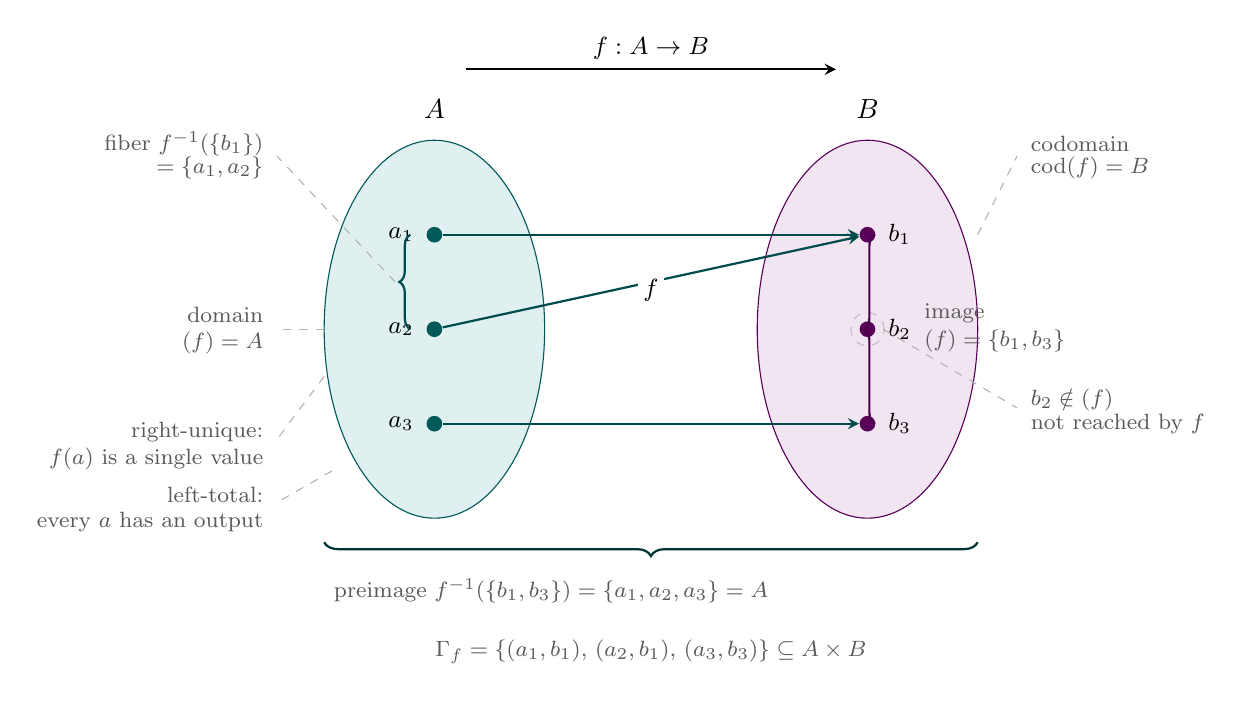
\begin{tikzpicture}[
    >=stealth,
    dot/.style     = {circle, fill, inner sep=2pt},
    teal/.style    = {draw=teal!70!black,  fill=teal!12},
    purple/.style  = {draw=violet!70!black, fill=violet!10},
    lbl/.style     = {font=\small},
    ann/.style     = {font=\footnotesize, text=gray!70!black},
    leader/.style  = {gray!60, dashed, thin},
    arr/.style     = {->, thick, teal!60!black},
    brace/.style   = {decorate,
                      decoration={brace, amplitude=4pt, raise=3pt},
                      thick, violet!60!black}
  ]
  \draw[teal]   (0,0)   ellipse (1.4cm and 2.4cm);
  \draw[purple] (5.5,0) ellipse (1.4cm and 2.4cm);

  \node[font=\normalsize\bfseries] at (0,    2.8) {$A$};
  \node[font=\normalsize\bfseries] at (5.5,  2.8) {$B$};

  \node[dot, teal!70!black] (a1) at (0,  1.2) {};
  \node[dot, teal!70!black] (a2) at (0,  0)   {};
  \node[dot, teal!70!black] (a3) at (0, -1.2) {};
  \node[lbl, left=4pt] at (a1) {$a_1$};
  \node[lbl, left=4pt] at (a2) {$a_2$};
  \node[lbl, left=4pt] at (a3) {$a_3$};

  \node[dot, violet!70!black] (b1) at (5.5,  1.2) {};
  \node[dot, violet!70!black] (b2) at (5.5,  0)   {};
  \node[dot, violet!70!black] (b3) at (5.5, -1.2) {};
  \node[lbl, right=4pt] at (b1) {$b_1$};
  \node[lbl, right=4pt] at (b2) {$b_2$};
  \node[lbl, right=4pt] at (b3) {$b_3$};

  \draw[gray!50, dashed, thin] (b2) circle (6pt);
  \draw[arr] (a1) -- (b1);
  \draw[arr] (a2) -- (b1);
  \draw[arr] (a3) -- (b3);
  \node[fill=white, inner sep=2pt, font=\small\bfseries] at (2.75, 0.5) {$f$};
  \draw[->, thick] (0.4, 3.3) -- node[above, font=\small\bfseries] {$f : A \to B$} (5.1, 3.3);

  \draw[leader] (-1.4, 0) -- (-2.0, 0);
  \node[ann, anchor=east] at (-2.05, 0.18) {domain};
  \node[ann, anchor=east] at (-2.05,-0.18) {$\dom(f) = A$};
  \draw[leader] (-1.3,-1.8) -- (-2.0,-2.2);
  \node[ann, anchor=east] at (-2.05,-2.1) {left-total:};
  \node[ann, anchor=east] at (-2.05,-2.45) {every $a$ has an output};
  \draw[leader] (-1.4, -0.6) -- (-2.0, -1.4);
  \node[ann, anchor=east] at (-2.05,-1.3)  {right-unique:};
  \node[ann, anchor=east] at (-2.05,-1.65) {$f(a)$ is a single value};

  \draw[leader] (6.9,  1.2) -- (7.4,  2.2);
  \node[ann, anchor=west] at (7.45, 2.35) {codomain};
  \node[ann, anchor=west] at (7.45, 2.05) {$\mathrm{cod}(f) = B$};
  \draw[brace] (5.7, -1.2) -- (5.7,  1.2);
  \node[ann, anchor=west] at (6.1,  0.2) {image};
  \node[ann, anchor=west] at (6.1, -0.15) {$\im(f) = \{b_1, b_3\}$};
  \draw[leader] (5.7, 0) -- (7.4, -1.0);
  \node[ann, anchor=west] at (7.45,-0.9)  {$b_2 \notin \im(f)$};
  \node[ann, anchor=west] at (7.45,-1.2)  {not reached by $f$};

  \draw[decorate,
        decoration={brace, amplitude=4pt, raise=3pt},
        thick, teal!60!black]
    (-0.2, 0) -- (-0.2, 1.2);
  \draw[leader] (-0.5, 0.6) -- (-2.0, 2.2);
  \node[ann, anchor=east] at (-2.05, 2.35) {fiber $f^{-1}(\{b_1\})$};
  \node[ann, anchor=east] at (-2.05, 2.05) {$= \{a_1, a_2\}$};

  \draw[decorate,
        decoration={brace, amplitude=5pt, raise=3pt, mirror},
        thick, teal!40!black]
    (-1.4,-2.6) -- (6.9,-2.6);
  \node[ann, anchor=north west] at (-1.4,-3.05)
    {preimage $f^{-1}(\{b_1,b_3\}) = \{a_1,a_2,a_3\} = A$};
  \node[ann] at (2.75,-4.1)
    {$\Gamma_f = \{(a_1,b_1),\,(a_2,b_1),\,(a_3,b_3)\} \subseteq A \times B$};
\end{tikzpicture}

  \caption{Vocabulary of a function $f:A\to B$.}
  \label{fig:function-vocabulary}
\end{figure}

\begin{remark*}[Interpretation]
A function assigns exactly one output in $B$ to every input in $A$.
In algebra, functions become structure-preserving objects when they are
required to respect specified operations, relations, or constants.
\end{remark*}

\begin{dependencies}
\begin{itemize}
  \item \hyperref[def:binary-relation]{Binary Relation}
  \item \hyperref[def:domain-codomain]{Domain and Codomain}
\end{itemize}
\end{dependencies}

\subsection*{Injective Functions}
\label{subsec:injective-functions}

\begin{definitionbox}{Definition (Injective)}
\begin{definition}[Injective Function]
\label{def:alg-injective}
Let $f:A\to B$.
The function $f$ is \textbf{injective} if
\[
\forall a_1,a_2 \in A,\;
f(a_1)=f(a_2) \Rightarrow a_1=a_2.
\]
\end{definition}
\end{definitionbox}

\begin{remark*}[Standard quantified statement]
\[
\operatorname{Injective}(f,A,B)
\Longleftrightarrow
f:A\to B
\land
\forall a_1,a_2\in A,\; f(a_1)=f(a_2)\Rightarrow a_1=a_2.
\]
\end{remark*}

\begin{remark*}[Definition predicate reading]
$f$ is injective exactly when equal outputs force equal inputs.
\end{remark*}

\begin{remark*}[Negated quantified statement]
\[
\neg\operatorname{Injective}(f,A,B)
\Longleftrightarrow
\exists a_1,a_2\in A,\;
a_1\neq a_2 \land f(a_1)=f(a_2).
\]
\end{remark*}

\begin{remark*}[Interpretation]
Injectivity means distinct inputs do not collide under the function.
\end{remark*}

\begin{dependencies}
\begin{itemize}
  \item \hyperref[def:alg-function]{Function}
\end{itemize}
\end{dependencies}

\subsection*{Surjective Functions}
\label{subsec:surjective-functions}

\begin{definitionbox}{Definition (Surjective)}
\begin{definition}[Surjective Function]
\label{def:alg-surjective}
Let $f:A\to B$.
The function $f$ is \textbf{surjective} if
\[
\forall b \in B,\; \exists a \in A,\; f(a)=b.
\]
\end{definition}
\end{definitionbox}

\begin{remark*}[Standard quantified statement]
\[
\operatorname{Surjective}(f,A,B)
\Longleftrightarrow
f:A\to B
\land
\forall b\in B,\; \exists a\in A,\; f(a)=b.
\]
\end{remark*}

\begin{remark*}[Definition predicate reading]
$f$ is surjective exactly when every element of the codomain is hit by some
input.
\end{remark*}

\begin{remark*}[Negated quantified statement]
\[
\neg\operatorname{Surjective}(f,A,B)
\Longleftrightarrow
\exists b\in B,\; \forall a\in A,\; f(a)\neq b.
\]
\end{remark*}

\begin{remark*}[Interpretation]
Surjectivity says that the image of $f$ fills the whole codomain.
\end{remark*}

\begin{dependencies}
\begin{itemize}
  \item \hyperref[def:alg-function]{Function}
\end{itemize}
\end{dependencies}

\subsection*{Bijective Functions}
\label{subsec:bijective-functions}

\begin{definitionbox}{Definition (Bijective)}
\begin{definition}[Bijective Function]
\label{def:alg-bijective}
Let $f:A\to B$.
The function $f$ is \textbf{bijective} if it is both injective and surjective.
\end{definition}
\end{definitionbox}

\begin{remark*}[Standard quantified statement]
\[
\operatorname{Bijective}(f,A,B)
\Longleftrightarrow
\operatorname{Injective}(f,A,B)\land \operatorname{Surjective}(f,A,B).
\]
\end{remark*}

\begin{remark*}[Definition predicate reading]
$f$ is bijective exactly when it is both injective and surjective.
\end{remark*}

\begin{remark*}[Negated quantified statement]
\[
\neg\operatorname{Bijective}(f,A,B)
\Longleftrightarrow
\neg\operatorname{Injective}(f,A,B)
\lor
\neg\operatorname{Surjective}(f,A,B).
\]
\end{remark*}

\begin{remark*}[Interpretation]
Bijectivity is the set-theoretic part of invertibility.  A bijective
structure-preserving map is the usual route to an isomorphism.
\end{remark*}

\begin{dependencies}
\begin{itemize}
  \item \hyperref[def:alg-injective]{Injective Function}
  \item \hyperref[def:alg-surjective]{Surjective Function}
\end{itemize}
\end{dependencies}

\subsection*{Morphisms}
\label{subsec:morphisms}

\begin{definitionbox}{Definition (Homomorphism)}
\begin{definition}[Homomorphism]
\label{def:algebraic-homomorphism}
Let $A$ and $B$ be algebraic structures of the same type.
A \textbf{homomorphism} $f:A\to B$ is a function that preserves the operations
of the structure.
\end{definition}
\end{definitionbox}

\begin{remark*}[Standard quantified statement]
\[
\operatorname{Homomorphism}(f,A,B)
\Longleftrightarrow
f:A\to B
\text{ and } f \text{ preserves the named operations of }A\text{ and }B.
\]
\end{remark*}

\begin{remark*}[Definition predicate reading]
$f$ is a homomorphism exactly when it is a structure-preserving function.
\end{remark*}

\begin{remark*}[Negated quantified statement]
\[
\neg\operatorname{Homomorphism}(f,A,B)
\]
when $f$ is not a function $A\to B$ or fails to preserve at least one named
operation.
\end{remark*}

\begin{remark*}[Interpretation]
Homomorphisms are the maps that keep algebraic operations visible through a
function.
\end{remark*}

\begin{dependencies}
\begin{itemize}
  \item \hyperref[def:alg-function]{Function}
  \item \hyperref[def:binary-operation]{Binary Operation}
\end{itemize}
\end{dependencies}

\begin{definition}[Monomorphism]
\label{def:monomorphism}
A \textbf{monomorphism} is an injective homomorphism.
\end{definition}

\begin{remark*}[Standard quantified statement]
\[
\operatorname{Monomorphism}(f,A,B)
\Longleftrightarrow
\operatorname{Homomorphism}(f,A,B)
\land
\operatorname{Injective}(f,A,B).
\]
\end{remark*}

\begin{remark*}[Definition predicate reading]
A monomorphism is a homomorphism that embeds without collisions.
\end{remark*}

\begin{remark*}[Negated quantified statement]
\[
\neg\operatorname{Monomorphism}(f,A,B)
\Longleftrightarrow
\neg\operatorname{Homomorphism}(f,A,B)
\lor
\neg\operatorname{Injective}(f,A,B).
\]
\end{remark*}

\begin{remark*}[Interpretation]
Monomorphisms preserve structure while keeping distinct inputs distinct.
\end{remark*}

\begin{dependencies}
\begin{itemize}
  \item \hyperref[def:algebraic-homomorphism]{Homomorphism}
  \item \hyperref[def:alg-injective]{Injective Function}
\end{itemize}
\end{dependencies}

\begin{definition}[Epimorphism]
\label{def:epimorphism}
An \textbf{epimorphism} is a surjective homomorphism.
\end{definition}

\begin{remark*}[Standard quantified statement]
\[
\operatorname{Epimorphism}(f,A,B)
\Longleftrightarrow
\operatorname{Homomorphism}(f,A,B)
\land
\operatorname{Surjective}(f,A,B).
\]
\end{remark*}

\begin{remark*}[Definition predicate reading]
An epimorphism is a homomorphism that reaches every element of the codomain.
\end{remark*}

\begin{remark*}[Negated quantified statement]
\[
\neg\operatorname{Epimorphism}(f,A,B)
\Longleftrightarrow
\neg\operatorname{Homomorphism}(f,A,B)
\lor
\neg\operatorname{Surjective}(f,A,B).
\]
\end{remark*}

\begin{remark*}[Interpretation]
Epimorphisms preserve structure while covering the whole target.
\end{remark*}

\begin{dependencies}
\begin{itemize}
  \item \hyperref[def:algebraic-homomorphism]{Homomorphism}
  \item \hyperref[def:alg-surjective]{Surjective Function}
\end{itemize}
\end{dependencies}

\begin{definition}[Isomorphism]
\label{def:isomorphism}
An \textbf{isomorphism} is a bijective homomorphism.
\end{definition}

\begin{remark*}[Standard quantified statement]
\[
\operatorname{Isomorphism}(f,A,B)
\Longleftrightarrow
\operatorname{Homomorphism}(f,A,B)
\land
\operatorname{Bijective}(f,A,B).
\]
\end{remark*}

\begin{remark*}[Definition predicate reading]
An isomorphism is a structure-preserving bijection.
\end{remark*}

\begin{remark*}[Negated quantified statement]
\[
\neg\operatorname{Isomorphism}(f,A,B)
\Longleftrightarrow
\neg\operatorname{Homomorphism}(f,A,B)
\lor
\neg\operatorname{Bijective}(f,A,B).
\]
\end{remark*}

\begin{remark*}[Interpretation]
Isomorphisms identify two structures as the same up to relabeling.
\end{remark*}

\begin{dependencies}
\begin{itemize}
  \item \hyperref[def:algebraic-homomorphism]{Homomorphism}
  \item \hyperref[def:alg-bijective]{Bijective Function}
\end{itemize}
\end{dependencies}

\begin{definition}[Endomorphism]
\label{def:endomorphism}
An \textbf{endomorphism} is a homomorphism from a structure to itself.
\end{definition}

\begin{remark*}[Standard quantified statement]
\[
\operatorname{Endomorphism}(f,A)
\Longleftrightarrow
\operatorname{Homomorphism}(f,A,A).
\]
\end{remark*}

\begin{remark*}[Definition predicate reading]
An endomorphism is a structure-preserving self-map.
\end{remark*}

\begin{remark*}[Negated quantified statement]
\[
\neg\operatorname{Endomorphism}(f,A)
\Longleftrightarrow
\neg\operatorname{Homomorphism}(f,A,A).
\]
\end{remark*}

\begin{remark*}[Interpretation]
Endomorphisms are internal symmetries or transformations, not necessarily
invertible ones.
\end{remark*}

\begin{dependencies}
\begin{itemize}
  \item \hyperref[def:algebraic-homomorphism]{Homomorphism}
\end{itemize}
\end{dependencies}

\begin{definition}[Automorphism]
\label{def:automorphism}
An \textbf{automorphism} is a bijective endomorphism.
\end{definition}

\begin{remark*}[Standard quantified statement]
\[
\operatorname{Automorphism}(f,A)
\Longleftrightarrow
\operatorname{Endomorphism}(f,A)
\land
\operatorname{Bijective}(f,A,A).
\]
\end{remark*}

\begin{remark*}[Definition predicate reading]
An automorphism is an invertible structure-preserving self-map.
\end{remark*}

\begin{remark*}[Negated quantified statement]
\[
\neg\operatorname{Automorphism}(f,A)
\Longleftrightarrow
\neg\operatorname{Endomorphism}(f,A)
\lor
\neg\operatorname{Bijective}(f,A,A).
\]
\end{remark*}

\begin{remark*}[Interpretation]
Automorphisms are the reversible symmetries of a structure.
\end{remark*}

\begin{dependencies}
\begin{itemize}
  \item \hyperref[def:endomorphism]{Endomorphism}
  \item \hyperref[def:alg-bijective]{Bijective Function}
\end{itemize}
\end{dependencies}


\section{Distinguished Elements}

\subsection*{Identity Elements}
\label{subsec:identity-elements}

\begin{definition}[Identity Element]
\label{def:identity-element}
Let $\star$ be a binary operation on $A$.
An element $e\in A$ is an \textbf{identity element} for $\star$ if
\[
\forall a\in A,\quad e\star a=a\star e=a.
\]
\end{definition}

\begin{remark*}[Standard quantified statement]
\[
\operatorname{IdentityElement}(e,\star,A)
\Longleftrightarrow
e\in A
\land
\forall a\in A,\; e\star a=a\star e=a.
\]
\end{remark*}

\begin{remark*}[Definition predicate reading]
$e$ is an identity for $\star$ exactly when multiplying by $e$ on either side
leaves every element unchanged.
\end{remark*}

\begin{remark*}[Negated quantified statement]
\[
\neg\operatorname{IdentityElement}(e,\star,A)
\Longleftrightarrow
e\notin A
\lor
\exists a\in A,\; e\star a\neq a \lor a\star e\neq a.
\]
\end{remark*}

\begin{remark*}[Interpretation]
An identity element is the distinguished element that does nothing under the
operation.
\end{remark*}

\begin{dependencies}
\begin{itemize}
  \item \hyperref[def:binary-operation]{Binary Operation}
\end{itemize}
\end{dependencies}

\begin{proposition}[Uniqueness of the Identity]
\label{prop:identity-element-unique}
In a group, the identity element is unique.
\hyperref[prf:group-identity-unique]{Go to proof.}
\end{proposition}

\begin{remark*}[Standard quantified statement]
\[
\operatorname{Group}(G,\star)
\Longrightarrow
\exists! e\in G\; \operatorname{IdentityElement}(e,\star,G).
\]
\end{remark*}

\begin{remark*}[Theorem predicate reading]
Every group has exactly one identity element.
\end{remark*}

\begin{remark*}[Negated quantified statement]
\[
\operatorname{Group}(G,\star)
\land
\exists e_1,e_2\in G,\;
\operatorname{IdentityElement}(e_1,\star,G)
\land
\operatorname{IdentityElement}(e_2,\star,G)
\land e_1\neq e_2
\Longrightarrow \bot.
\]
\end{remark*}

\begin{remark*}[Interpretation]
The symbol for the identity is not extra arbitrary data once the group
operation is fixed.
\end{remark*}

\begin{dependencies}
\begin{itemize}
  \item \hyperref[def:algebraic-group]{Group}
  \item \hyperref[def:identity-element]{Identity Element}
\end{itemize}
\end{dependencies}

\begin{remark*}[Proof TODO]
Regenerate this proof as a one-proof-per-file artifact.
\end{remark*}

\subsection*{Inverses}
\label{subsec:inverses}

\begin{definition}[Inverse Element]
\label{def:inverse-element}
Let $\star$ be a binary operation on $A$ with identity element $e$.
An element $b\in A$ is an \textbf{inverse} of $a\in A$ if
\[
a\star b=b\star a=e.
\]
\end{definition}

\begin{remark*}[Standard quantified statement]
\[
\operatorname{InverseElement}(b,a,\star,e,G)
\Longleftrightarrow
a,b,e\in G
\land
a\star b=b\star a=e.
\]
\end{remark*}

\begin{remark*}[Definition predicate reading]
$b$ is an inverse of $a$ exactly when composing $a$ and $b$ in either order
returns the identity.
\end{remark*}

\begin{remark*}[Negated quantified statement]
\[
\neg\operatorname{InverseElement}(b,a,\star,e,G)
\Longleftrightarrow
b\notin G
\lor
a\star b\neq e
\lor
b\star a\neq e.
\]
\end{remark*}

\begin{remark*}[Interpretation]
An inverse is an element that undoes another element with respect to the group
operation.
\end{remark*}

\begin{dependencies}
\begin{itemize}
  \item \hyperref[def:binary-operation]{Binary Operation}
  \item \hyperref[def:identity-element]{Identity Element}
\end{itemize}
\end{dependencies}

\begin{proposition}[Uniqueness of Inverses]
\label{prop:inverse-element-unique}
In a group, every element has a unique inverse.
\hyperref[prf:group-inverse-unique]{Go to proof.}
\end{proposition}

\begin{remark*}[Standard quantified statement]
\[
\operatorname{Group}(G,\star)
\Longrightarrow
\forall a\in G,\; \exists! b\in G\;
\operatorname{InverseElement}(b,a,\star,e,G).
\]
\end{remark*}

\begin{remark*}[Theorem predicate reading]
Every element of a group has exactly one inverse.
\end{remark*}

\begin{remark*}[Negated quantified statement]
\[
\operatorname{Group}(G,\star)
\land
\exists a,b,c\in G,\;
\operatorname{InverseElement}(b,a,\star,e,G)
\land
\operatorname{InverseElement}(c,a,\star,e,G)
\land b\neq c
\Longrightarrow \bot.
\]
\end{remark*}

\begin{remark*}[Interpretation]
Once the group operation and identity are fixed, inverse notation is
well-defined.
\end{remark*}

\begin{dependencies}
\begin{itemize}
  \item \hyperref[def:algebraic-group]{Group}
  \item \hyperref[def:inverse-element]{Inverse Element}
  \item \hyperref[def:identity-element]{Identity Element}
\end{itemize}
\end{dependencies}

\begin{remark*}[Proof TODO]
Regenerate this proof as a one-proof-per-file artifact.
\end{remark*}

\subsection*{Absorbing Elements}
\label{subsec:absorbing-elements}

\begin{definition}[Absorbing Element]
\label{def:algebraic-absorbing-element}
Let $\star$ be a binary operation on $A$.
An element $z\in A$ is an \textbf{absorbing element} for $\star$ if
\[
\forall a\in A,\quad z\star a=a\star z=z.
\]
\end{definition}

\begin{remark*}[Standard quantified statement]
\[
\operatorname{AbsorbingElement}(z,\star,A)
\Longleftrightarrow
z\in A
\land
\forall a\in A,\; z\star a=a\star z=z.
\]
\end{remark*}

\begin{remark*}[Definition predicate reading]
$z$ is absorbing for $\star$ exactly when combining any element with $z$ on
either side returns $z$.
\end{remark*}

\begin{remark*}[Negated quantified statement]
\[
\neg\operatorname{AbsorbingElement}(z,\star,A)
\Longleftrightarrow
z\notin A
\lor
\exists a\in A,\; z\star a\neq z \lor a\star z\neq z.
\]
\end{remark*}

\begin{remark*}[Interpretation]
An absorbing element collapses every product involving it back to itself.
\end{remark*}

\begin{remark*}[Examples]
The element $0$ is absorbing for multiplication in the integers, reals, and
complex numbers.
\end{remark*}

\begin{dependencies}
\begin{itemize}
  \item \hyperref[def:binary-operation]{Binary Operation}
\end{itemize}
\end{dependencies}

\subsection*{Distinguished Constants}
\label{subsec:distinguished-constants}

\begin{remark*}[Exposition]
Distinguished constants are the model-theoretic presentation of named elements.
The group identity $e$, additive identity $0$, and multiplicative identity $1$
are constants when they are part of the signature.
\end{remark*}


\section{Algebraic Structures}

\subsection*{Structure Signatures}
\label{subsec:structure-signatures}

\begin{definitionbox}{Definition (First-Order Signature)}
\begin{definition}[First-Order Signature]
\label{def:first-order-signature}
A \textbf{first-order signature} $\mathcal{L}$ consists of constant symbols,
function symbols with specified arities, and relation symbols with specified
arities.
\end{definition}
\end{definitionbox}

\begin{remark*}[Standard quantified statement]
\[
\mathcal{L}=(\mathrm{Const}_{\mathcal{L}},
\mathrm{Func}_{\mathcal{L}},
\mathrm{Rel}_{\mathcal{L}},\operatorname{arity})
\]
where each function and relation symbol has a specified arity.
\end{remark*}

\begin{remark*}[Definition predicate reading]
A first-order signature is the syntactic list of symbols that a structure must
interpret.
\end{remark*}

% Omitted Negated quantified statement: a signature is specified data, not a
% predicate whose negation is useful here.

\begin{remark*}[Interpretation]
The signature describes what kinds of constants, operations, and relations are
visible before any particular carrier set is chosen.
\end{remark*}

\begin{dependencies}
\begin{itemize}
  \item \hyperref[def:nullary-operation]{Nullary Operation}
  \item \hyperref[def:unary-operation]{Unary Operation}
  \item \hyperref[def:binary-operation]{Binary Operation}
  \item \hyperref[def:binary-relation]{Binary Relation}
\end{itemize}
\end{dependencies}

\begin{definitionbox}{Definition ($\mathcal{L}$-Structure)}
\begin{definition}[$\mathcal{L}$-Structure]
\label{def:algebraic-l-structure}
Given a signature $\mathcal{L}$, an \textbf{$\mathcal{L}$-structure}
$\mathcal{A}$ consists of a nonempty carrier set $A$ together with
interpretations of each constant, function, and relation symbol of
$\mathcal{L}$ on $A$.
\end{definition}
\end{definitionbox}

\begin{remark*}[Standard quantified statement]
\[
\mathcal{A}\models\mathcal{L}
\Longleftrightarrow
\mathcal{A}=(A,\ldots)
\text{ interprets each symbol of }\mathcal{L}\text{ on }A.
\]
\end{remark*}

\begin{remark*}[Definition predicate reading]
$\mathcal{A}$ is an $\mathcal{L}$-structure exactly when it gives meanings to
the symbols of $\mathcal{L}$ on a carrier set.
\end{remark*}

\begin{remark*}[Negated quantified statement]
\[
\neg\operatorname{Structure}_{\mathcal{L}}(\mathcal{A})
\]
when some symbol of $\mathcal{L}$ is not interpreted with the required arity on
the carrier set.
\end{remark*}

\begin{remark*}[Interpretation]
The signature is the type; the structure is the instance.  A group signature
names multiplication, identity, and inverse, while a particular group
interprets those symbols on a carrier set.
\end{remark*}

\begin{dependencies}
\begin{itemize}
  \item \hyperref[def:first-order-signature]{First-Order Signature}
  \item \hyperref[def:carrier-set]{Carrier Set}
\end{itemize}
\end{dependencies}

\subsection*{Magmas}
\label{subsec:magmas}

\begin{definitionbox}{Definition (Magma)}
\begin{definition}[Magma]
\label{def:magma}
A \textbf{magma} is a pair $(A,\star)$ where $A$ is a nonempty set and
$\star:A\times A\to A$ is a binary operation.
\end{definition}
\end{definitionbox}

\begin{remark*}[Standard quantified statement]
\[
\operatorname{Magma}(A,\star)
\Longleftrightarrow
A\neq\varnothing
\land
\operatorname{BinaryOperation}(\star,A).
\]
\end{remark*}

\begin{remark*}[Definition predicate reading]
$(A,\star)$ is a magma exactly when $A$ is nonempty and $\star$ is closed on
$A$.
\end{remark*}

\begin{remark*}[Negated quantified statement]
\[
\neg\operatorname{Magma}(A,\star)
\Longleftrightarrow
A=\varnothing
\lor
\neg\operatorname{BinaryOperation}(\star,A).
\]
\end{remark*}

\begin{remark*}[Interpretation]
A magma is the weakest nontrivial algebraic structure: it has a carrier set and
a closed binary operation, with no associativity, identity, inverse, or
commutativity requirements.
\end{remark*}

\begin{dependencies}
\begin{itemize}
  \item \hyperref[def:carrier-set]{Carrier Set}
  \item \hyperref[def:binary-operation]{Binary Operation}
\end{itemize}
\end{dependencies}

\subsection*{Semigroups}
\label{subsec:semigroups}

\begin{definitionbox}{Definition (Semigroup)}
\begin{definition}[Semigroup]
\label{def:algebraic-semigroup}
A \textbf{semigroup} is a pair $(A,\star)$ where $A$ is a nonempty set and
$\star:A\times A\to A$ is an associative binary operation:
\[
\forall a,b,c \in A,\quad
(a\star b)\star c=a\star(b\star c).
\]
\end{definition}
\end{definitionbox}

\begin{remark*}[Standard quantified statement]
\[
\operatorname{Semigroup}(A,\star)
\Longleftrightarrow
\operatorname{Magma}(A,\star)
\land
\operatorname{Associative}(\star,A).
\]
\end{remark*}

\begin{remark*}[Definition predicate reading]
$(A,\star)$ is a semigroup exactly when it is a magma whose operation is
associative.
\end{remark*}

\begin{remark*}[Negated quantified statement]
\[
\neg\operatorname{Semigroup}(A,\star)
\Longleftrightarrow
\neg\operatorname{Magma}(A,\star)
\lor
\neg\operatorname{Associative}(\star,A).
\]
\end{remark*}

\begin{remark*}[Interpretation]
Semigroups are magmas where finite products can be written without specifying
parentheses.
\end{remark*}

\begin{remark*}[Examples]
Nonempty strings under concatenation and positive integers under addition are
standard semigroups.
\end{remark*}

\begin{dependencies}
\begin{itemize}
  \item \hyperref[def:magma]{Magma}
  \item \hyperref[def:algebraic-associativity]{Associativity}
\end{itemize}
\end{dependencies}

\subsection*{Monoids}
\label{subsec:monoids}

\begin{definitionbox}{Definition (Monoid)}
\begin{definition}[Monoid]
\label{def:algebraic-monoid}
A \textbf{monoid} is a triple $(A,\star,e)$ where $(A,\star)$ is a semigroup
and $e\in A$ is an identity element:
\[
\forall a \in A,\quad a\star e=e\star a=a.
\]
\end{definition}
\end{definitionbox}

\begin{remark*}[Standard quantified statement]
\[
\operatorname{Monoid}(A,\star,e)
\Longleftrightarrow
\operatorname{Semigroup}(A,\star)
\land
\operatorname{IdentityElement}(e,\star,A).
\]
\end{remark*}

\begin{remark*}[Definition predicate reading]
$(A,\star,e)$ is a monoid exactly when $(A,\star)$ is a semigroup and $e$ is a
two-sided identity for $\star$.
\end{remark*}

\begin{remark*}[Negated quantified statement]
\[
\neg\operatorname{Monoid}(A,\star,e)
\Longleftrightarrow
\neg\operatorname{Semigroup}(A,\star)
\lor
\neg\operatorname{IdentityElement}(e,\star,A).
\]
\end{remark*}

\begin{remark*}[Interpretation]
Monoids add a do-nothing element to associative composition.
\end{remark*}

\begin{remark*}[Examples]
The natural numbers under addition with identity $0$, the natural numbers under
multiplication with identity $1$, and strings under concatenation with the
empty string are monoids.
\end{remark*}

\begin{dependencies}
\begin{itemize}
  \item \hyperref[def:algebraic-semigroup]{Semigroup}
  \item \hyperref[def:identity-element]{Identity Element}
\end{itemize}
\end{dependencies}

\subsection*{Groups}
\label{subsec:groups}

\begin{definitionbox}{Definition (Group)}
\begin{definition}[Group]
\label{def:algebraic-group}
A \textbf{group} is a pair $(G,\star)$ where $G$ is a set and $\star$ is a
binary operation on $G$ satisfying:
\begin{enumerate}[label=\textbf{G\arabic*.}]
  \item associativity;
  \item existence of an identity element $e\in G$;
  \item existence, for each $a\in G$, of an inverse element $a^{-1}\in G$.
\end{enumerate}
\end{definition}
\end{definitionbox}

\begin{remark*}[Standard quantified statement]
\[
\operatorname{Group}(G,\star)
\Longleftrightarrow
\exists e\in G,\;
\operatorname{Monoid}(G,\star,e)
\land
\forall a\in G,\;\exists b\in G\;
\operatorname{InverseElement}(b,a,\star,e,G).
\]
\end{remark*}

\begin{remark*}[Definition predicate reading]
$(G,\star)$ is a group exactly when it is an associative closed operation with
an identity and an inverse for every element.
\end{remark*}

\begin{remark*}[Negated quantified statement]
\[
\neg\operatorname{Group}(G,\star)
\Longleftrightarrow
\neg\operatorname{Associative}(\star,G)
\lor
\text{no two-sided identity exists}
\lor
\text{some element has no two-sided inverse}.
\]
\end{remark*}

\begin{remark*}[Interpretation]
Groups are algebraic structures of reversible composition.
\end{remark*}

\begin{dependencies}
\begin{itemize}
  \item \hyperref[def:binary-operation]{Binary Operation}
  \item \hyperref[def:algebraic-associativity]{Associativity}
  \item \hyperref[def:identity-element]{Identity Element}
  \item \hyperref[def:inverse-element]{Inverse Element}
\end{itemize}
\end{dependencies}

\begin{definition}[Order of a Group]
\label{def:order-of-a-group}
The \textbf{order} of a group $G$, denoted $|G|$, is the cardinality of its
underlying set.  If $|G|$ is finite, $G$ is a finite group; otherwise it is an
infinite group.
\end{definition}

\begin{remark*}[Standard quantified statement]
\[
\operatorname{OrderOfGroup}(G)=|G|.
\]
\end{remark*}

\begin{remark*}[Definition predicate reading]
The order of $G$ is the number of elements in the carrier set of $G$.
\end{remark*}

% Omitted Negated quantified statement: this definition introduces notation for
% a cardinal value rather than a predicate with a useful failure condition.

\begin{remark*}[Interpretation]
Finite groups are classified by a natural-number order; infinite groups have
infinite cardinal order.
\end{remark*}

\begin{remark*}[Examples]
Examples include $(\mathbb{Z},+)$, $(\mathbb{Q}\setminus\{0\},\cdot)$,
$(\mathbb{Z}/n\mathbb{Z},+)$, and $GL_n(\mathbb{R})$ under matrix
multiplication.
\end{remark*}

\begin{dependencies}
\begin{itemize}
  \item \hyperref[def:algebraic-group]{Group}
  \item TODO: formalize cardinality.
\end{itemize}
\end{dependencies}

\subsection*{Abelian Groups}
\label{subsec:abelian-groups}

\begin{definitionbox}{Definition (Abelian Group)}
\begin{definition}[Abelian Group]
\label{def:algebraic-abelian-group}
A group $(G,\star)$ is \textbf{abelian} if its operation is commutative:
\[
\forall a,b \in G,\quad a\star b=b\star a.
\]
\end{definition}
\end{definitionbox}

\begin{remark*}[Standard quantified statement]
\[
\operatorname{AbelianGroup}(G,\star)
\Longleftrightarrow
\operatorname{Group}(G,\star)
\land
\operatorname{Commutative}(\star,G).
\]
\end{remark*}

\begin{remark*}[Definition predicate reading]
$(G,\star)$ is abelian exactly when it is a group whose operation commutes.
\end{remark*}

\begin{remark*}[Negated quantified statement]
\[
\neg\operatorname{AbelianGroup}(G,\star)
\Longleftrightarrow
\neg\operatorname{Group}(G,\star)
\lor
\exists a,b\in G,\; a\star b\neq b\star a.
\]
\end{remark*}

\begin{remark*}[Interpretation]
Abelian groups are usually written additively: the operation is $+$, the
identity is $0$, and the inverse of $a$ is $-a$.
\end{remark*}

\begin{dependencies}
\begin{itemize}
  \item \hyperref[def:algebraic-group]{Group}
  \item \hyperref[def:algebraic-commutativity]{Commutativity}
\end{itemize}
\end{dependencies}

\subsection*{Rings}
\label{subsec:rings}

\begin{definitionbox}{Definition (Ring)}
\begin{definition}[Ring]
\label{def:algebraic-ring}
A \textbf{ring} is a triple $(R,+,\cdot)$ where $R$ is a set and $+$ and
$\cdot$ are binary operations on $R$ satisfying:
\begin{enumerate}[label=\textbf{R\arabic*.}]
  \item $(R,+)$ is an abelian group;
  \item multiplication is associative;
  \item multiplication distributes over addition on the left and on the right.
\end{enumerate}
\end{definition}
\end{definitionbox}

\begin{remark*}[Standard quantified statement]
\[
\operatorname{Ring}(R,+,\cdot)
\Longleftrightarrow
\operatorname{AbelianGroup}(R,+)
\land
\operatorname{Associative}(\cdot,R)
\land
\operatorname{LeftDistributive}(\cdot,+,R)
\land
\operatorname{RightDistributive}(\cdot,+,R).
\]
\end{remark*}

\begin{remark*}[Definition predicate reading]
$(R,+,\cdot)$ is a ring exactly when addition forms an abelian group,
multiplication is associative, and multiplication distributes over addition.
\end{remark*}

\begin{remark*}[Negated quantified statement]
\[
\neg\operatorname{Ring}(R,+,\cdot)
\Longleftrightarrow
\neg\operatorname{AbelianGroup}(R,+)
\lor
\neg\operatorname{Associative}(\cdot,R)
\lor
\neg\operatorname{LeftDistributive}(\cdot,+,R)
\lor
\neg\operatorname{RightDistributive}(\cdot,+,R).
\]
\end{remark*}

\begin{remark*}[Interpretation]
A ring is the algebraic setting where addition, subtraction, and multiplication
coexist coherently.
\end{remark*}

\begin{dependencies}
\begin{itemize}
  \item \hyperref[def:algebraic-abelian-group]{Abelian Group}
  \item \hyperref[def:algebraic-associativity]{Associativity}
  \item \hyperref[def:algebraic-left-distributivity]{Left Distributivity}
  \item \hyperref[def:algebraic-right-distributivity]{Right Distributivity}
\end{itemize}
\end{dependencies}

\begin{definition}[Commutative Ring]
\label{def:algebraic-commutative-ring}
A ring $(R,+,\cdot)$ is \textbf{commutative} if
\[
\forall a,b \in R,\quad a\cdot b=b\cdot a.
\]
\end{definition}

\begin{remark*}[Standard quantified statement]
\[
\operatorname{CommutativeRing}(R,+,\cdot)
\Longleftrightarrow
\operatorname{Ring}(R,+,\cdot)
\land
\operatorname{Commutative}(\cdot,R).
\]
\end{remark*}

\begin{remark*}[Definition predicate reading]
A ring is commutative exactly when its multiplication commutes.
\end{remark*}

\begin{remark*}[Negated quantified statement]
\[
\neg\operatorname{CommutativeRing}(R,+,\cdot)
\Longleftrightarrow
\neg\operatorname{Ring}(R,+,\cdot)
\lor
\exists a,b\in R,\; a\cdot b\neq b\cdot a.
\]
\end{remark*}

\begin{remark*}[Interpretation]
Commutative rings are rings whose multiplication behaves symmetrically in its
two inputs.
\end{remark*}

\begin{dependencies}
\begin{itemize}
  \item \hyperref[def:algebraic-ring]{Ring}
  \item \hyperref[def:algebraic-commutativity]{Commutativity}
\end{itemize}
\end{dependencies}

\begin{definition}[Ring with Unity]
\label{def:algebraic-ring-with-unity}
A ring $(R,+,\cdot)$ is a \textbf{ring with unity} if there exists
$1\in R$ such that
\[
\forall a \in R,\quad 1\cdot a=a\cdot 1=a.
\]
\end{definition}

\begin{remark*}[Standard quantified statement]
\[
\operatorname{RingWithUnity}(R,+,\cdot,1)
\Longleftrightarrow
\operatorname{Ring}(R,+,\cdot)
\land
\operatorname{IdentityElement}(1,\cdot,R).
\]
\end{remark*}

\begin{remark*}[Definition predicate reading]
A ring has unity exactly when multiplication has a two-sided identity.
\end{remark*}

\begin{remark*}[Negated quantified statement]
\[
\neg\operatorname{RingWithUnity}(R,+,\cdot,1)
\Longleftrightarrow
\neg\operatorname{Ring}(R,+,\cdot)
\lor
\neg\operatorname{IdentityElement}(1,\cdot,R).
\]
\end{remark*}

\begin{remark*}[Interpretation]
The unity element is the multiplicative identity of the ring.
\end{remark*}

\begin{remark*}[Examples]
The integers, residue rings $\mathbb{Z}/n\mathbb{Z}$, polynomial rings, and
matrix rings are standard examples of rings.
\end{remark*}

\begin{dependencies}
\begin{itemize}
  \item \hyperref[def:algebraic-ring]{Ring}
  \item \hyperref[def:identity-element]{Identity Element}
\end{itemize}
\end{dependencies}

\subsection*{Integral Domains}
\label{subsec:integral-domains}

\begin{definition*}[Zero Divisor]
Let $R$ be a ring.
A nonzero element $a\in R$ is a \textbf{zero divisor} if there exists a
nonzero element $b\in R$ such that $ab=0$.
\end{definition*}

\begin{remark*}[Canonical reference]
The canonical dependency label for this vocabulary is
\hyperref[def:zero-divisor]{Zero Divisor} in Volume~II.
\end{remark*}

\begin{remark*}[Standard quantified statement]
\[
\operatorname{ZeroDivisor}(a,R)
\Longleftrightarrow
a\in R
\land a\neq 0
\land
\exists b\in R,\; b\neq 0 \land ab=0.
\]
\end{remark*}

\begin{remark*}[Definition predicate reading]
$a$ is a zero divisor exactly when a nonzero multiplication by $a$ can produce
zero.
\end{remark*}

\begin{remark*}[Negated quantified statement]
\[
\neg\operatorname{ZeroDivisor}(a,R)
\Longleftrightarrow
a=0
\lor
\forall b\in R,\; ab=0 \Rightarrow b=0.
\]
\end{remark*}

\begin{remark*}[Interpretation]
Zero divisors identify where multiplication loses cancellation behavior.
\end{remark*}

\begin{dependencies}
\begin{itemize}
  \item \hyperref[def:algebraic-ring]{Ring}
  \item \hyperref[def:algebraic-absorbing-element]{Absorbing Element}
\end{itemize}
\end{dependencies}

\begin{definitionbox}{Definition (Integral Domain)}
\begin{definition}[Integral Domain]
\label{def:algebraic-integral-domain}
An \textbf{integral domain} is a commutative ring with unity in which there are
no zero divisors.
\end{definition}
\end{definitionbox}

\begin{remark*}[Standard quantified statement]
\[
\operatorname{IntegralDomain}(R,+,\cdot,0,1)
\Longleftrightarrow
\operatorname{CommutativeRing}(R,+,\cdot)
\land
\operatorname{RingWithUnity}(R,+,\cdot,1)
\land
\forall a,b\in R,\; ab=0 \Rightarrow a=0 \lor b=0.
\]
\end{remark*}

\begin{remark*}[Definition predicate reading]
An integral domain is a commutative ring with $1$ where a product is zero only
because at least one factor is zero.
\end{remark*}

\begin{remark*}[Negated quantified statement]
\[
\neg\operatorname{IntegralDomain}(R,+,\cdot,0,1)
\Longleftrightarrow
\neg\operatorname{CommutativeRing}(R,+,\cdot)
\lor
\neg\operatorname{RingWithUnity}(R,+,\cdot,1)
\lor
\exists a,b\in R,\; a\neq0\land b\neq0\land ab=0.
\]
\end{remark*}

\begin{remark*}[Interpretation]
Integral domains are the commutative rings where multiplication has no nonzero
zero-divisor obstruction.
\end{remark*}

\begin{dependencies}
\begin{itemize}
  \item \hyperref[def:algebraic-commutative-ring]{Commutative Ring}
  \item \hyperref[def:algebraic-ring-with-unity]{Ring with Unity}
  \item \hyperref[def:zero-divisor]{Zero Divisor}
\end{itemize}
\end{dependencies}

\begin{proposition}[Cancellation in Integral Domains]
\label{prop:abstract-domain-cancellation}
Let $R$ be an integral domain.  If $a\neq 0$ and $ab=ac$, then $b=c$.
\hyperref[prf:domain-cancellation]{Go to proof.}
\end{proposition}

\begin{remark*}[Standard quantified statement]
\[
\operatorname{IntegralDomain}(R)
\Longrightarrow
\forall a,b,c\in R,\; a\neq0 \land ab=ac \Rightarrow b=c.
\]
\end{remark*}

\begin{remark*}[Theorem predicate reading]
Nonzero factors can be cancelled in an integral domain.
\end{remark*}

\begin{remark*}[Negated quantified statement]
\[
\operatorname{IntegralDomain}(R)
\land
\exists a,b,c\in R,\; a\neq0 \land ab=ac \land b\neq c
\Longrightarrow \bot.
\]
\end{remark*}

\begin{remark*}[Interpretation]
Cancellation is recovered in integral domains because nonzero elements are not
zero divisors.
\end{remark*}

\begin{dependencies}
\begin{itemize}
  \item \hyperref[def:algebraic-integral-domain]{Integral Domain}
  \item \hyperref[def:zero-divisor]{Zero Divisor}
\end{itemize}
\end{dependencies}

\begin{remark*}[Proof TODO]
Regenerate this proof as a one-proof-per-file artifact.
\end{remark*}

\subsection*{Fields}
\label{subsec:fields}

\begin{definitionbox}{Definition (Field)}
\begin{definition}[Field]
\label{def:algebraic-field}
A \textbf{field} is a set $F$ equipped with two binary operations, addition
$+$ and multiplication $\cdot$, such that:
\begin{enumerate}[label=\textbf{F\arabic*.}]
  \item $(F,+)$ is an abelian group with identity $0$;
  \item $F\setminus\{0\}$ is an abelian group under multiplication with
        identity $1$;
  \item multiplication distributes over addition.
\end{enumerate}
\end{definition}
\end{definitionbox}

\begin{remark*}[Standard quantified statement]
\[
\operatorname{Field}(F,+,\cdot,0,1)
\Longleftrightarrow
\operatorname{AbelianGroup}(F,+)
\land
\operatorname{AbelianGroup}(F\setminus\{0\},\cdot)
\land
\operatorname{LeftDistributive}(\cdot,+,F)
\land
\operatorname{RightDistributive}(\cdot,+,F).
\]
\end{remark*}

\begin{remark*}[Definition predicate reading]
A field is an additive abelian group whose nonzero elements form a
multiplicative abelian group, with multiplication distributing over addition.
\end{remark*}

\begin{remark*}[Negated quantified statement]
\[
\neg\operatorname{Field}(F,+,\cdot,0,1)
\Longleftrightarrow
\neg\operatorname{AbelianGroup}(F,+)
\lor
\neg\operatorname{AbelianGroup}(F\setminus\{0\},\cdot)
\lor
\neg\operatorname{LeftDistributive}(\cdot,+,F)
\lor
\neg\operatorname{RightDistributive}(\cdot,+,F).
\]
\end{remark*}

\begin{remark*}[Interpretation]
Fields are the algebraic setting where addition, subtraction, multiplication,
and division by nonzero elements are all available.
\end{remark*}

\begin{dependencies}
\begin{itemize}
  \item \hyperref[def:algebraic-abelian-group]{Abelian Group}
  \item \hyperref[def:algebraic-left-distributivity]{Left Distributivity}
  \item \hyperref[def:algebraic-right-distributivity]{Right Distributivity}
\end{itemize}
\end{dependencies}

\begin{proposition}[Every Field is an Integral Domain]
\label{prop:abstract-field-is-domain}
Every field is an integral domain.
\hyperref[prf:field-is-domain]{Go to proof.}
\end{proposition}

\begin{remark*}[Standard quantified statement]
\[
\operatorname{Field}(F,+,\cdot,0,1)
\Longrightarrow
\operatorname{IntegralDomain}(F,+,\cdot,0,1).
\]
\end{remark*}

\begin{remark*}[Theorem predicate reading]
The field axioms imply the integral-domain axioms.
\end{remark*}

\begin{remark*}[Negated quantified statement]
\[
\operatorname{Field}(F,+,\cdot,0,1)
\land
\neg\operatorname{IntegralDomain}(F,+,\cdot,0,1)
\Longrightarrow \bot.
\]
\end{remark*}

\begin{remark*}[Interpretation]
The existence of inverses for nonzero elements prevents nonzero zero divisors.
\end{remark*}

\begin{dependencies}
\begin{itemize}
  \item \hyperref[def:algebraic-field]{Field}
  \item \hyperref[def:algebraic-integral-domain]{Integral Domain}
  \item \hyperref[def:inverse-element]{Inverse Element}
\end{itemize}
\end{dependencies}

\begin{remark*}[Proof TODO]
Regenerate this proof as a one-proof-per-file artifact.
\end{remark*}


% =========================================================
% Groups
% =========================================================
\section{Groups}

% =========================================================
% Binary Operations
% =========================================================
\paragraph{Binary Operations}


% =========================================================
% Binary Operations --- Notes
% =========================================================

% ---------------------------------------------------------
% Definition --- Binary Operation
% ---------------------------------------------------------

\begin{definitionbox}{Definition (Binary Operation)}
\begin{definition}[Binary Operation]
\label{def:algebraic-group-binary-operation}
Let $G$ be a set. A \textbf{binary operation} on $G$ is a function
\[
\star : G \times G \to G.
\]
For $a, b \in G$, the element $\star(a,b)$ is denoted by $a \star b$.
\end{definition}
\end{definitionbox}

\begin{remark*}[Standard quantified statement]
\[
\begin{aligned}
&\star \text{ is a binary operation on } G \\
&\quad\Longleftrightarrow\quad
\forall a \in G\;\forall b \in G,\; a \star b \in G.
\end{aligned}
\]
\end{remark*}

\begin{remark*}[Definition predicate reading]
\[
\operatorname{BinaryOperation}(\star, G)
\;\colonequiv\;
\forall a \in G\;\forall b \in G,\; a \star b \in G.
\]
\end{remark*}

\begin{remark*}[Negated quantified statement]
\[
\begin{aligned}
&\star \text{ is not a binary operation on } G \\
&\quad\Longleftrightarrow\quad
\exists a \in G\;\exists b \in G \text{ such that } a \star b \notin G.
\end{aligned}
\]
\end{remark*}

\begin{remark*}[Negation predicate reading]
\[
\neg \operatorname{BinaryOperation}(\star, G)
\;\colonequiv\;
\exists a \in G\;\exists b \in G \text{ such that } a \star b \notin G.
\]
\end{remark*}

\begin{remark*}[Failure modes]
\[
\exists a \in G\;\exists b \in G \text{ such that } a \star b \notin G.
\]
\end{remark*}

\begin{remark*}[Failure mode decomposition]
\[
\begin{aligned}
&\star \text{ fails to be a binary operation on } G \\
&\quad\Longleftrightarrow\quad
\exists a \in G\;\exists b \in G \text{ such that } a \star b \notin G.
\end{aligned}
\]
\end{remark*}

\begin{remark*}[Interpretation]
A binary operation takes two elements of $G$ and returns another element of $G$.
This encodes closure of the operation within the set.
\end{remark*}

% ---------------------------------------------------------
% Definition --- Associativity
% ---------------------------------------------------------

\begin{definitionbox}{Definition (Associativity)}
\begin{definition}[Associativity]
\label{def:algebraic-group-associativity}
Let $\star$ be a binary operation on $G$. The operation $\star$ is
\textbf{associative} if
\[
(a \star b) \star c = a \star (b \star c)
\quad \text{for all } a, b, c \in G.
\]
\end{definition}
\end{definitionbox}

\begin{remark*}[Standard quantified statement]
\[
\begin{aligned}
&\star \text{ is associative on } G \\
&\quad\Longleftrightarrow\quad
\forall a \in G\;\forall b \in G\;\forall c \in G,\;
(a \star b) \star c = a \star (b \star c).
\end{aligned}
\]
\end{remark*}

\begin{remark*}[Definition predicate reading]
\[
\operatorname{Associative}(\star, G)
\;\colonequiv\;
\forall a \in G\;\forall b \in G\;\forall c \in G,\;
(a \star b) \star c = a \star (b \star c).
\]
\end{remark*}

\begin{remark*}[Negated quantified statement]
\[
\begin{aligned}
&\star \text{ is not associative on } G \\
&\quad\Longleftrightarrow\quad
\exists a \in G\;\exists b \in G\;\exists c \in G \text{ such that } \\
&\qquad (a \star b) \star c \ne a \star (b \star c).
\end{aligned}
\]
\end{remark*}

\begin{remark*}[Negation predicate reading]
\[
\neg \operatorname{Associative}(\star, G)
\;\colonequiv\;
\exists a \in G\;\exists b \in G\;\exists c \in G \text{ such that }
(a \star b) \star c \ne a \star (b \star c).
\]
\end{remark*}

\begin{remark*}[Failure modes]
\[
\exists a \in G\;\exists b \in G\;\exists c \in G \text{ such that }
(a \star b) \star c \ne a \star (b \star c).
\]
\end{remark*}

\begin{remark*}[Failure mode decomposition]
\[
\begin{aligned}
&\star \text{ fails associativity} \\
&\quad\Longleftrightarrow\quad
\exists a,b,c \in G \text{ witnessing a parenthesization mismatch.}
\end{aligned}
\]
\end{remark*}

\begin{remark*}[Interpretation]
Associativity means that the way elements are grouped does not affect the result.
\end{remark*}

% ---------------------------------------------------------
% Definition --- Commutativity
% ---------------------------------------------------------

\begin{definitionbox}{Definition (Commutativity)}
\begin{definition}[Commutativity]
\label{def:algebraic-group-commutativity}
Let $\star$ be a binary operation on $G$. The operation $\star$ is
\textbf{commutative} if
\[
a \star b = b \star a
\quad \text{for all } a, b \in G.
\]
\end{definition}
\end{definitionbox}

\begin{remark*}[Standard quantified statement]
\[
\begin{aligned}
&\star \text{ is commutative on } G \\
&\quad\Longleftrightarrow\quad
\forall a \in G\;\forall b \in G,\; a \star b = b \star a.
\end{aligned}
\]
\end{remark*}

\begin{remark*}[Definition predicate reading]
\[
\operatorname{Commutative}(\star, G)
\;\colonequiv\;
\forall a \in G\;\forall b \in G,\; a \star b = b \star a.
\]
\end{remark*}

\begin{remark*}[Negated quantified statement]
\[
\begin{aligned}
&\star \text{ is not commutative on } G \\
&\quad\Longleftrightarrow\quad
\exists a \in G\;\exists b \in G \text{ such that } a \star b \ne b \star a.
\end{aligned}
\]
\end{remark*}

\begin{remark*}[Negation predicate reading]
\[
\neg \operatorname{Commutative}(\star, G)
\;\colonequiv\;
\exists a \in G\;\exists b \in G \text{ such that } a \star b \ne b \star a.
\]
\end{remark*}

\begin{remark*}[Failure modes]
\[
\exists a \in G\;\exists b \in G \text{ such that } a \star b \ne b \star a.
\]
\end{remark*}

\begin{remark*}[Failure mode decomposition]
\[
\begin{aligned}
&\star \text{ fails commutativity} \\
&\quad\Longleftrightarrow\quad
\exists a,b \in G \text{ where swapping inputs changes the result.}
\end{aligned}
\]
\end{remark*}

\begin{remark*}[Interpretation]
Commutativity means the order of the inputs does not affect the result.
\end{remark*}

% ---------------------------------------------------------
% Remark --- Relationship
% ---------------------------------------------------------

\begin{remark*}[Interpretation]
Associativity and commutativity are independent properties. For example,
addition on $\mathbb{Z}$ is both associative and commutative; matrix
multiplication is associative but not commutative; subtraction on
$\mathbb{Z}$ is neither.
\end{remark*}
































% =========================================================
% Group Definition and Axioms
% =========================================================
\paragraph{Definition of a Group}

\begin{definition}[Group]
\label{def:notes-groups-definition-l6}
A \emph{group} is a pair $(G, \star)$ where $G$ is a set and
$\star$ is a binary operation on $G$ satisfying the following axioms:

\begin{enumerate}[label=\textbf{G\arabic*.}]
  \item \textbf{Associativity.}
        $(a \star b) \star c = a \star (b \star c)$
        for all $a, b, c \in G$.

  \item \textbf{Identity.}
        There exists an element $e \in G$ such that
        \[
          e \star a = a \star e = a
          \quad \text{for all } a \in G.
        \]
        The element $e$ is called the \emph{identity element} of $G$.

  \item \textbf{Inverses.}
        For each $a \in G$, there exists an element $a^{-1} \in G$ such that
        \[
          a \star a^{-1} = a^{-1} \star a = e.
        \]
        The element $a^{-1}$ is called the \emph{inverse} of $a$.
\end{enumerate}
\end{definition}

\begin{remark}
Closure is not listed as a separate axiom because it is already
encoded in the requirement that $\star : G \times G \to G$ is a
binary operation --- the codomain forces the result to stay in $G$.

Intuitively: a group is a set where you can combine elements,
undo combinations, and the order of grouping never matters.
\end{remark}

\begin{remark}[Axiom Count]
Some treatments list four axioms (closure, associativity, identity, inverses).
Here closure is absorbed into the definition of binary operation,
leaving three axioms. Both presentations define the same object.
\end{remark}

\begin{remark}[Notation]
When the operation is understood from context, we write $ab$ instead
of $a \star b$, and call $G$ itself a group rather than the pair $(G, \star)$.
For groups whose operation is addition, we write $a + b$, use $0$ for the
identity, and $-a$ for the inverse of $a$.
\end{remark}

\begin{definition}[Order of a Group]
\label{def:notes-groups-definition-l54}
The \emph{order} of a group $G$, denoted $|G|$, is the cardinality of $G$
as a set. If $|G|$ is finite, $G$ is called a \emph{finite group};
otherwise it is an \emph{infinite group}.
\end{definition}

\begin{example}[Canonical Examples of Groups]
\begin{enumerate}[label=(\roman*)]
  \item $(\mathbb{Z}, +)$: the integers under addition.
        Identity: $0$. Inverse of $n$: $-n$. Infinite group.

  \item $(\mathbb{Q} \setminus \{0\}, \cdot)$: nonzero rationals under multiplication.
        Identity: $1$. Inverse of $q$: $1/q$. Infinite group.

  \item $(\mathbb{Z}/n\mathbb{Z}, +)$: integers modulo $n$ under addition.
        Identity: $[0]$. Inverse of $[k]$: $[n-k]$. Finite group of order $n$.

  \item $(GL_n(\mathbb{R}), \cdot)$: invertible $n \times n$ real matrices
        under multiplication.
        Identity: $I_n$. Inverse: matrix inverse. Infinite group.
\end{enumerate}
\end{example}

\begin{remark}
Note what fails to be a group:
$(\mathbb{Z}, \cdot)$ is not a group because $2$ has no multiplicative
inverse in $\mathbb{Z}$.
$(\mathbb{N}, +)$ is not a group because positive integers have no
additive inverse in $\mathbb{N}$.
These failures illustrate why each axiom is necessary.
\end{remark}

% =========================================================
% Basic Theorems of Groups
% =========================================================
\paragraph{Basic Theorems}

\begin{remark}[Why These Theorems Matter]
The group axioms guarantee existence of an identity and inverses,
but say nothing about uniqueness. The following theorems establish
that both are unique. This is essential: without uniqueness, we
cannot speak of \emph{the} identity or \emph{the} inverse of an element,
and proofs that equate two objects via the identity or inverse would
be invalid.

These same uniqueness theorems reappear in vector space proofs,
where they are cited by name. They are proved once here.
\end{remark}

% ---------------------------------------------------------
\begin{proposition}[Uniqueness of the Identity]
\label{prop:group-identity-unique}
Let $G$ be a group. The identity element of $G$ is unique.
\hyperref[prf:group-identity-unique]{Go to proof.}
\end{proposition}

\begin{remark*}
\FlashQ{State uniqueness of the group identity.}
\FlashA{In any group $G$, the identity element is unique.}
\FlashHint{If $e,e\'$ are both identities: $e=e\cdot e\'=e\'$.}
\end{remark*}



\begin{remark}
The proof strategy is standard for uniqueness arguments:
assume two identities exist, then show they must be equal.
This pattern recurs throughout algebra whenever a definition
asserts existence of a distinguished element.

Intuitively: if two elements both act as an identity,
applying one to the other forces them to coincide.
\end{remark}

% ---------------------------------------------------------
\begin{proposition}[Uniqueness of Inverses]
\label{prop:group-inverse-unique}
Let $G$ be a group. For each $a \in G$, the inverse of $a$ is unique.
\hyperref[prf:group-inverse-unique]{Go to proof.}
\end{proposition}

\begin{remark*}
\FlashQ{State uniqueness of group inverses.}
\FlashA{In any group $G$, each element has a unique inverse.}
\FlashHint{If $b$ and $c$ are both inverses of $a$: $b=b(ac)=(ba)c=c$.}
\end{remark*}



\begin{remark}
Intuitively: if two elements both undo $a$, then they must be
the same element --- because each can be obtained from the other
by cancellation.
\end{remark}

% ---------------------------------------------------------
\begin{proposition}[Cancellation Laws]
\label{prop:group-cancellation-in-groups}
Let $G$ be a group and let $a, b, c \in G$. Then:
\begin{enumerate}[label=(\roman*)]
  \item \textbf{Left cancellation:} $ab = ac \implies b = c$.
  \item \textbf{Right cancellation:} $ba = ca \implies b = c$.
\end{enumerate}
\hyperref[prf:group-cancellation]{Go to proof.}
\end{proposition}


\begin{remark}
Cancellation is what makes group equations solvable.
It does \emph{not} hold in general for rings or monoids without inverses.

Intuitively: multiply both sides by $a^{-1}$ and the common factor disappears.
\end{remark}

% ---------------------------------------------------------
\begin{proposition}[Socks-Shoes Property]
\label{prop:group-socks-shoes}
Let $G$ be a group and let $a, b \in G$. Then
\[
(ab)^{-1} = b^{-1} a^{-1}.
\]
\hyperref[prf:group-socks-shoes]{Go to proof.}
\end{proposition}

\begin{remark*}
\FlashQ{State the Socks-Shoes Property.}
\FlashA{$(ab)^{-1} = b^{-1}a^{-1}$.}
\FlashHint{Verify directly: $(ab)(b^{-1}a^{-1}) = a(bb^{-1})a^{-1} = e$.}
\FlashNeg{$(ab)^{-1} \neq a^{-1}b^{-1}$ in general for non-abelian groups.}
\end{remark*}


\begin{remark}
The name comes from the observation that to undo putting on socks
then shoes, you must first remove the shoes, then the socks ---
in reverse order.

This reversal of order is characteristic of non-abelian groups and
becomes important in the theory of group homomorphisms and
in matrix algebra, where $(AB)^{-1} = B^{-1}A^{-1}$.
\end{remark}

% =========================================================
% Abelian Groups
% =========================================================
\paragraph{Abelian Groups}

\begin{definition}[Abelian Group]
\label{def:notes-groups-abelian-l6}
A group $(G, \star)$ is called \emph{abelian} (or \emph{commutative}) if
\[
a \star b = b \star a \quad \text{for all } a, b \in G.
\]
\end{definition}

\begin{remark}
An abelian group is a group with one additional axiom: commutativity
of the operation. Every abelian group is a group, but not every group
is abelian.

Intuitively: in an abelian group, the order in which you combine
elements is irrelevant. This is the familiar arithmetic of addition
on $\mathbb{Z}$, $\mathbb{Q}$, $\mathbb{R}$, and $\mathbb{C}$.
\end{remark}

\begin{remark}[Structural Position]
Abelian groups are the additive backbone of every vector space.
The four vector space axioms governing addition --- associativity,
commutativity, existence of zero, existence of additive inverses ---
are precisely the axioms that make $(V, +)$ an abelian group.

This is why the vector space definition can be stated compactly as:
\emph{a vector space over $\mathbb{F}$ is an abelian group $(V,+)$
equipped with a scalar multiplication by $\mathbb{F}$}.
The abelian group structure is not an analogy; it is the literal
algebraic content of the first four vector space axioms.
\end{remark}

\begin{example}[Abelian and Non-Abelian Groups]
\begin{enumerate}[label=(\roman*)]
  \item $(\mathbb{Z}, +)$, $(\mathbb{R}, +)$, $(\mathbb{C}, +)$:
        all abelian. These are the additive groups underlying the
        standard vector spaces.

  \item $(\mathbb{Z}/n\mathbb{Z}, +)$: abelian for all $n \geq 1$.

  \item $(GL_n(\mathbb{R}), \cdot)$ for $n \geq 2$: \emph{not} abelian,
        since matrix multiplication does not commute in general.

  \item $(S_n, \circ)$ for $n \geq 3$: the symmetric group on $n$ symbols
        under composition is not abelian.
\end{enumerate}
\end{example}

\begin{remark}[Additive Notation Convention]
For abelian groups, it is standard to write the operation as $+$,
the identity as $0$, and the inverse of $a$ as $-a$.
This additive notation is used throughout linear algebra, where
$(V, +)$ is always an abelian group.
\end{remark}













% =========================================================
% Rings
% =========================================================
\section{Rings}

% =========================================================
% Ring Definition and Axioms
% =========================================================
\paragraph{Definition of a Ring}

\begin{remark}[Motivation]
A group has one binary operation. A ring has two: addition and
multiplication. The addition makes the ring an abelian group.
Multiplication is layered on top, connected to addition through
the distributive laws.

Rings are the natural algebraic home of arithmetic. The integers
$\mathbb{Z}$, polynomials $\mathbb{Z}[x]$, and square matrices
$M_n(\mathbb{R})$ are all rings. What they share is not the
specific objects but the axiom structure --- and every theorem
proved here holds simultaneously in all of them.
\end{remark}

\begin{definition}[Ring]
\label{def:notes-rings-definition-l19}
A \emph{ring} is a triple $(R, +, \cdot)$ where $R$ is a set and
$+$ and $\cdot$ are binary operations on $R$ satisfying:

\begin{enumerate}[label=\textbf{R\arabic*.}]
  \item \textbf{Additive abelian group.}
        $(R, +)$ is an abelian group:
        \begin{itemize}
          \item $(a + b) + c = a + (b + c)$ for all $a,b,c \in R$.
          \item $a + b = b + a$ for all $a, b \in R$.
          \item There exists $0 \in R$ such that $a + 0 = a$ for all $a \in R$.
          \item For each $a \in R$, there exists $-a \in R$ such that
                $a + (-a) = 0$.
        \end{itemize}

  \item \textbf{Multiplicative associativity.}
        $(a \cdot b) \cdot c = a \cdot (b \cdot c)$
        for all $a, b, c \in R$.

  \item \textbf{Distributivity.}
        \begin{itemize}
          \item $a \cdot (b + c) = a \cdot b + a \cdot c$
                for all $a,b,c \in R$.
          \item $(a + b) \cdot c = a \cdot c + b \cdot c$
                for all $a,b,c \in R$.
        \end{itemize}
\end{enumerate}
\end{definition}

\begin{remark}[What a Ring Does and Does Not Require]
A ring does \emph{not} require:
\begin{itemize}
  \item commutativity of multiplication ($ab = ba$ need not hold),
  \item a multiplicative identity ($1$ need not exist),
  \item multiplicative inverses ($a^{-1}$ need not exist).
\end{itemize}
Each additional requirement produces a richer structure.
A ring with a multiplicative identity is a \emph{ring with unity}.
A commutative ring with unity where every nonzero element has a
multiplicative inverse is a \emph{field} --- covered in the next section.

Intuitively: a ring is the minimal structure needed for addition,
subtraction, and multiplication to coexist and interact sensibly.
Division is not guaranteed.
\end{remark}

\begin{definition}[Commutative Ring]
\label{def:notes-rings-definition-l65}
A ring $(R, +, \cdot)$ is \emph{commutative} if
\[
a \cdot b = b \cdot a \quad \text{for all } a, b \in R.
\]
\end{definition}

\begin{definition}[Ring with Unity]
\label{def:notes-rings-definition-l72}
A ring $(R, +, \cdot)$ is a \emph{ring with unity} if there exists
$1 \in R$ such that
\[
1 \cdot a = a \cdot 1 = a \quad \text{for all } a \in R.
\]
The element $1$ is called the \emph{multiplicative identity} or \emph{unity}.
When it exists, it is unique (proof identical to
Proposition~\ref{prop:group-identity-unique} applied to $(R, \cdot)$).
\end{definition}

\begin{example}[Canonical Examples of Rings]
\begin{enumerate}[label=(\roman*)]
  \item $(\mathbb{Z}, +, \cdot)$: integers.
        Commutative ring with unity $1$.
        No multiplicative inverses for $|n| \neq 1$.

  \item $(\mathbb{Z}/n\mathbb{Z}, +, \cdot)$: integers modulo $n$.
        Commutative ring with unity $[1]$.

  \item $(M_n(\mathbb{R}), +, \cdot)$: $n \times n$ real matrices.
        Ring with unity $I_n$. \emph{Not} commutative for $n \geq 2$.

  \item $(\mathbb{Z}[x], +, \cdot)$: polynomials with integer coefficients.
        Commutative ring with unity $1$.

  \item The trivial ring $\{0\}$, where $0 = 1$, is the only ring
        in which the additive and multiplicative identities coincide.
\end{enumerate}
\end{example}

% =========================================================
% Basic Theorems of Rings
% =========================================================
\paragraph{Basic Theorems}

\begin{remark}[What Needs Proving]
The ring axioms say nothing explicitly about how multiplication
interacts with the additive identity $0$ or with additive inverses.
These must be derived. The key tool in both proofs is distributivity
--- the bridge between the two operations.

Notice that these proofs make no assumption about which ring you are in.
They work in $\mathbb{Z}$, in $M_n(\mathbb{R})$, in $\mathbb{Z}[x]$,
in any ring simultaneously.
\end{remark}

\begin{proposition}[Multiplication by Zero]
\label{prop:ring-mult-zero}
Let $R$ be a ring. For all $a \in R$,
\[
a \cdot 0 = 0 \cdot a = 0.
\]
\hyperref[prf:ring-mult-zero]{Go to proof.}
\end{proposition}

\begin{remark*}
\FlashQ{State: multiplication by zero in a ring.}
\FlashA{In any ring $R$: $a\cdot 0=0\cdot a=0$ for all $a\in R$.}
\FlashHint{Distributivity: $a\cdot 0=a(0+0)=a\cdot 0+a\cdot 0$; cancel by additive inverse.}
\end{remark*}



\begin{remark}
The proof uses distributivity to produce the equation
$a \cdot 0 + a \cdot 0 = a \cdot 0$, then applies additive
cancellation to conclude $a \cdot 0 = 0$.

This is not circular: $0$ on the left side is the additive identity
of the ring; the $0$ on the right is the same element being derived
as a consequence of cancellation. The proof works because additive
cancellation was already proved for all abelian groups
(Proposition~\ref{prop:group-cancellation}).
\end{remark}

\begin{proposition}[Multiplication by Additive Inverse]
\label{prop:ring-mult-neg}
Let $R$ be a ring. For all $a, b \in R$,
\[
a \cdot (-b) = -(a \cdot b)
\quad\text{and}\quad
(-a) \cdot b = -(a \cdot b).
\]
In any ring with unity, $(-1) \cdot a = -a$.
\hyperref[prf:ring-mult-neg]{Go to proof.}
\end{proposition}

\begin{remark*}
\FlashQ{In a ring, what is $a \cdot (-b)$?}
\FlashA{$a(-b) = -(ab)$ and $(-a)b = -(ab)$; in a ring with unity $(-1)a = -a$.}
\FlashHint{Show $a(-b)$ satisfies the defining property of $-(ab)$, then invoke uniqueness of additive inverse.}
\end{remark*}


\begin{remark}
The proof strategy is: show $a \cdot (-b)$ satisfies the defining
property of the additive inverse of $a \cdot b$, then invoke
uniqueness of additive inverses
(Proposition~\ref{prop:group-inverse-unique}).

This is the same strategy used in the vector space proof that
$(-1)v = -v$ --- because that proof is just this theorem applied
to the scalar field $\mathbb{F}$ acting on $V$.
\end{remark}

% =========================================================
% Integral Domains
% =========================================================
\paragraph{Integral Domains}

\begin{remark}[Motivation]
In $\mathbb{Z}$, if $ab = 0$ then $a = 0$ or $b = 0$.
This feels obvious but it is not an axiom of rings --- it fails in
$\mathbb{Z}/6\mathbb{Z}$, where $[2] \cdot [3] = [0]$ even though
neither $[2]$ nor $[3]$ is zero. Elements that behave like $[2]$
and $[3]$ are called zero divisors, and rings without them are
integral domains.

This property matters because it is exactly what is needed for
multiplicative cancellation --- and for the zero product argument
that appears throughout linear algebra.
\end{remark}

\begin{definition}[Zero Divisor]
\label{def:notes-rings-integral-domains-l19}
Let $R$ be a commutative ring with unity.
A nonzero element $a \in R$ is a \emph{zero divisor} if there exists
a nonzero $b \in R$ such that $a \cdot b = 0$.
\end{definition}

\begin{definition}[Integral Domain]
\label{def:notes-rings-integral-domains-l25}
A commutative ring with unity $R$ is an \emph{integral domain} if
$R$ has no zero divisors. Equivalently,
\[
a \cdot b = 0 \;\Longrightarrow\; a = 0 \;\text{ or }\; b = 0
\quad \text{for all } a, b \in R.
\]
\end{definition}

\begin{remark}[Connection to Linear Algebra]
The zero product property is the theorem cited in the vector space proof
that $av = \mathbf{0} \Rightarrow a = 0$ or $v = \mathbf{0}$.
Specifically, the case $a \neq 0$ uses the fact that the scalar field
$\mathbb{F}$ has no zero divisors --- which holds because every field
is an integral domain (proved in the next section).

The proof is not about vectors at all. It is about the scalar field.
\end{remark}

\begin{proposition}[Cancellation in Integral Domains]
\label{prop:domain-cancellation}
Let $R$ be an integral domain and $a, b, c \in R$ with $a \neq 0$.
Then
\[
ab = ac \;\Longrightarrow\; b = c.
\]
\hyperref[prf:domain-cancellation]{Go to proof.}
\end{proposition}

\begin{remark*}
\FlashQ{State cancellation in an integral domain.}
\FlashA{In integral domain $R$: $a \neq 0$ and $ab = ac \Rightarrow b = c$.}
\FlashHint{$ab = ac \Rightarrow a(b-c) = 0$; since $a \neq 0$ and no zero divisors, $b - c = 0$.}
\FlashNeg{Fails in $\mathbb{Z}/6\mathbb{Z}$: $2 \cdot 1 = 2 \cdot 4 = 2$ but $1 \neq 4$.}
\end{remark*}


\begin{example}[Integral Domains and Non-Examples]
\begin{enumerate}[label=(\roman*)]
  \item $\mathbb{Z}$, $\mathbb{Q}$, $\mathbb{R}$, $\mathbb{C}$:
        all integral domains.
  \item $\mathbb{Z}[x]$: integral domain.
  \item $\mathbb{Z}/p\mathbb{Z}$ for prime $p$: integral domain
        (in fact a field, as shown in the next section).
  \item $\mathbb{Z}/6\mathbb{Z}$: \emph{not} an integral domain,
        since $[2][3] = [0]$ with $[2],[3] \neq [0]$.
  \item $M_2(\mathbb{R})$: \emph{not} an integral domain ---
        not commutative, and admits zero divisors.
\end{enumerate}
\end{example}

% =========================================================
% Boolean Rings
% =========================================================
\paragraph{Boolean Rings}

\begin{definitionbox}{Definition --- Boolean Ring}
\begin{definition}[Boolean Ring]
\label{def:boolean-ring}
A \textbf{Boolean ring} is a ring with unity $(R,+,\cdot,1)$ such that
every element is idempotent under multiplication:
\[
  \tag{B1}
  p\cdot p = p \quad \text{for every } p\in R.
\]
\end{definition}
\end{definitionbox}

\begin{remark*}[Standard quantified statement]
\[
\operatorname{BooleanRing}(R,+,\cdot,1)
\Longleftrightarrow
\operatorname{RingWithUnity}(R,+,\cdot,1)
\land
\forall p\in R,\; p\cdot p=p.
\]
\end{remark*}

\begin{remark*}[Definition predicate reading]
$(R,+,\cdot,1)$ is a Boolean ring exactly when it is a ring with a
multiplicative identity whose multiplication is idempotent.
\end{remark*}

\begin{remark*}[Negated quantified statement]
\[
\neg\operatorname{BooleanRing}(R,+,\cdot,1)
\Longleftrightarrow
\neg\operatorname{RingWithUnity}(R,+,\cdot,1)
\;\lor\;
\exists p\in R,\; p\cdot p\neq p.
\]
\end{remark*}

\begin{remark*}[Rewire note]
This definition reuses
\hyperref[def:idempotent-operation]{Idempotent Operation}:
\[
  \operatorname{BooleanRing}(R,+,\cdot,1)
  \Longleftrightarrow
  \operatorname{RingWithUnity}(R,+,\cdot,1)
  \land
  \operatorname{IdempotentOperation}(\cdot,R).
\]
There is no separate idempotent-element predicate here; the Boolean
condition is idempotence of multiplication as an operation.
\end{remark*}

\begin{remark*}[Characteristic 2 is derived, not assumed]
Some presentations list $p+p=0$ as an axiom of Boolean rings. In this
volume it is a theorem, Proposition~\ref{prop:boolean-ring-self-additive-inverse}.
Thus
\[
  \operatorname{BooleanRing}(R,+,\cdot,1)
  \Longrightarrow
  \operatorname{Characteristic2}(R,+).
\]
\end{remark*}

\begin{proposition}[Self Additive Inverse / Characteristic 2]
\label{prop:boolean-ring-self-additive-inverse}
In any Boolean ring $R$,
\[
  p+p=0 \quad \text{for every } p\in R.
\]
\hyperref[prf:boolean-ring-self-additive-inverse]{Go to proof.}
\end{proposition}

\begin{remark*}
\FlashQ{What is the additive characteristic of a Boolean ring?}
\FlashA{Every element satisfies $p+p=0$; Boolean rings have characteristic $2$ unless they are trivial.}
\FlashHint{Apply idempotence to $(p+q)^2$ and cancel the shared $p$ and $q$ terms.}
\end{remark*}

\begin{proposition}[Self Negation]
\label{prop:boolean-ring-self-negation}
In any Boolean ring $R$,
\[
  -p=p \quad \text{for every } p\in R.
\]
\hyperref[prf:boolean-ring-self-negation]{Go to proof.}
\end{proposition}

\begin{proposition}[Commutativity from Idempotence]
\label{prop:boolean-ring-commutativity-from-idempotence}
In any Boolean ring $R$,
\[
  pq=qp \quad \text{for all } p,q\in R.
\]
Hence every Boolean ring is a commutative ring
(Definition~\ref{def:notes-rings-definition-l65}).
\hyperref[prf:boolean-ring-commutativity-from-idempotence]{Go to proof.}
\end{proposition}

\begin{remark}[Structural Link to Integral Domains]
\label{rem:boolean-rings-and-integral-domains}
Every Boolean ring with more than two elements has zero divisors, hence
is not an integral domain (Definition~\ref{def:notes-rings-integral-domains-l25}).
Indeed, idempotence gives
\[
  p(1-p)=p-p^2=p-p=0.
\]
If $p\neq 0$ and $p\neq 1$, then $p$ and $1-p$ are nonzero zero divisors.
The only Boolean ring that is an integral domain is the two-element ring
$\mathbf{2}\cong\mathbb{F}_2$.
\end{remark}

\begin{example}[Standard Boolean Rings]
\label{ex:boolean-ring-standard-examples}
\begin{enumerate}[label=(\roman*)]
  \item The two-element ring
        \[
          \mathbf{2}=\{0,1\}
        \]
        with addition and multiplication modulo $2$ is a Boolean ring.
        Its operation tables are
        \[
        \begin{array}{c|cc}
        + & 0 & 1\\ \hline
        0 & 0 & 1\\
        1 & 1 & 0
        \end{array}
        \qquad
        \begin{array}{c|cc}
        \cdot & 0 & 1\\ \hline
        0 & 0 & 0\\
        1 & 0 & 1
        \end{array}
        \]
        and both elements satisfy $p^2=p$.

  \item For any $n\geq 1$, the product ring $\mathbf{2}^n$ with
        coordinatewise addition and multiplication is a Boolean ring.
        The four-element case $\mathbf{2}^2$ has elements
        $(0,0),(1,0),(0,1),(1,1)$, and idempotence holds coordinatewise:
        \[
          (a,b)^2=(a^2,b^2)=(a,b).
        \]

  \item For any set $X$, the power set
        \[
          \bigl(\mathcal P(X),\triangle,\cap,X\bigr)
        \]
        is a Boolean ring. Addition is symmetric difference, multiplication
        is intersection, the zero element is $\varnothing$, and the unity is
        $X$. This example is isomorphic to the function ring $\mathbf{2}^{X}$.
\end{enumerate}
\end{example}

\begin{theorem}[Stone Representation for Boolean Rings, stated]
\label{thm:stone-representation-boolean-rings}
Every Boolean ring is isomorphic to a field of sets. Every finite Boolean
ring is isomorphic to $\mathcal P(X)$ for some finite set $X$, hence has
$2^{|X|}$ elements.
\hyperref[prf:stone-representation-boolean-rings]{Go to proof.}
\end{theorem}

\begin{corollary}[Order is a Power of Two]
\label{cor:boolean-ring-finite-order-power-two}
A finite Boolean ring has order $2^n$ for some $n\geq 0$. In particular,
there is no Boolean ring of order $3$.
\hyperref[prf:boolean-ring-finite-order-power-two]{Go to proof.}
\end{corollary}

\begin{remark*}[Placement note]
The representation theorem is recorded here so the Boolean-ring facts stay
contiguous. A later abstract-algebra chapter may move the proof once ideals,
prime ideals, and ultrafilters are available.
\end{remark*}


% =========================================================
% Fields
% =========================================================
\section{Fields}

% =========================================================
% Field Definition and Axioms
% =========================================================
\paragraph{Definition of a Field}

\begin{remark}[Motivation]
A ring allows addition, subtraction, and multiplication.
A field adds division: every nonzero element has a multiplicative inverse.
This is the structure of $\mathbb{Q}$, $\mathbb{R}$, and $\mathbb{C}$ ---
the number systems where you can always solve $ax = b$ for $a \neq 0$.

Fields are the scalars of linear algebra. Axler's $\mathbb{F}$ denotes
an arbitrary field, meaning every theorem in linear algebra holds
simultaneously over $\mathbb{R}$, $\mathbb{C}$, $\mathbb{Q}$,
and any other field --- because the proofs use only field axioms,
not properties specific to real or complex numbers.
\end{remark}

\begin{definition}[Field]
\label{def:notes-fields-definition-l19}
A \emph{field} is a commutative ring with unity $(F, +, \cdot)$
satisfying:

\begin{enumerate}[label=\textbf{F\arabic*.}]
  \item \textbf{Additive abelian group.}
        $(F, +)$ is an abelian group with identity $0$.

  \item \textbf{Multiplicative abelian group on nonzero elements.}
        $(F \setminus \{0\}, \cdot)$ is an abelian group with identity $1$.
        Explicitly: for each $a \in F$ with $a \neq 0$, there exists
        $a^{-1} \in F$ such that $a \cdot a^{-1} = 1$.

  \item \textbf{Distributivity.}
        $a \cdot (b + c) = a \cdot b + a \cdot c$
        for all $a, b, c \in F$.

  \item \textbf{Non-triviality.}
        $0 \neq 1$.
\end{enumerate}
\end{definition}

\begin{remark}[Unpacking the Definition]
A field is simultaneously:
\begin{itemize}
  \item $(F, +)$: an abelian group (additive structure),
  \item $(F \setminus \{0\}, \cdot)$: an abelian group (multiplicative structure),
  \item connected by distributivity.
\end{itemize}
The non-triviality axiom $0 \neq 1$ rules out the trivial ring $\{0\}$,
which would otherwise technically satisfy the other axioms.
\end{remark}

\begin{example}[Fields]
\begin{enumerate}[label=(\roman*)]
  \item $\mathbb{Q}$, $\mathbb{R}$, $\mathbb{C}$: the standard fields.
  \item $\mathbb{Z}/p\mathbb{Z}$ for any prime $p$: a finite field
        with $p$ elements, denoted $\mathbb{F}_p$.
  \item $\mathbb{Q}(\sqrt{2}) = \{a + b\sqrt{2} : a, b \in \mathbb{Q}\}$:
        a field extending $\mathbb{Q}$.
\end{enumerate}
\end{example}

\begin{example}[Non-Fields]
\begin{enumerate}[label=(\roman*)]
  \item $\mathbb{Z}$: not a field. The element $2$ has no multiplicative
        inverse in $\mathbb{Z}$.
  \item $\mathbb{Z}/6\mathbb{Z}$: not a field. $[2]$ has no inverse
        since $\gcd(2,6) \neq 1$. (Also not an integral domain.)
  \item $M_n(\mathbb{R})$ for $n \geq 2$: not a field.
        Not commutative, and singular matrices have no inverse.
\end{enumerate}
\end{example}

% =========================================================
% Basic Theorems of Fields
% =========================================================
\paragraph{Basic Theorems}

\begin{remark}[Why These Theorems Matter]
These are the theorems cited in every vector space proof that crosses
from the scalar side to the vector side. They live here, in the field,
and are cited by number when needed in linear algebra.
\end{remark}

\begin{proposition}[Every Field is an Integral Domain]
\label{prop:field-is-domain}
Every field is an integral domain.
\hyperref[prf:field-is-domain]{Go to proof.}
\end{proposition}

\begin{remark*}
\FlashQ{State: every field is an integral domain.}
\FlashA{Every field is an integral domain: $ab=0\Rightarrow a=0$ or $b=0$.}
\FlashHint{If $a\neq 0$, multiply by $a^{-1}$ to get $b=0$.}
\FlashNeg{$\mathbb{Z}/6\mathbb{Z}$ is a ring but not a domain: $2\cdot 3=0$.}
\end{remark*}



\begin{remark}
This is the theorem behind the linear algebra argument:
if $av = \mathbf{0}$ and $a \neq 0$, then $v = \mathbf{0}$.
The scalar $a$ lives in a field $\mathbb{F}$, and the key step
is that $\mathbb{F}$ has no zero divisors.
\end{remark}

\begin{proposition}[Zero Product Property in a Field]
\label{prop:field-zero-product}
Let $\mathbb{F}$ be a field and $a, b \in \mathbb{F}$. Then
\[
ab = 0 \;\Longrightarrow\; a = 0 \;\text{ or }\; b = 0.
\]
\hyperref[prf:field-zero-product]{Go to proof.}
\end{proposition}

\begin{remark*}
\FlashQ{State the zero-product property in a field.}
\FlashA{In field $\mathbb{F}$: $ab=0\Rightarrow a=0$ or $b=0$.}
\FlashHint{If $a\neq 0$ multiply by $a^{-1}$.}
\FlashNeg{Fails in $\mathbb{Z}/6\mathbb{Z}$: $2\cdot 3=0$.}
\end{remark*}




\begin{proposition}[Nonzero Scalars Have Inverses]
\label{prop:field-inverse-exists}
Let $\mathbb{F}$ be a field and $a \in \mathbb{F}$ with $a \neq 0$.
Then there exists a unique $a^{-1} \in \mathbb{F}$ such that
$a \cdot a^{-1} = 1$.
\hyperref[prf:field-inverse-exists]{Go to proof.}
\end{proposition}

\begin{remark*}
\FlashQ{State uniqueness of multiplicative inverses in a field.}
\FlashA{For $a\neq 0$ in field $\mathbb{F}$, there is a unique $a^{-1}$ with $a\cdot a^{-1}=1$.}
\FlashHint{If $ax=ay=1$ then $x=x(ay)=(xa)y=y$.}
\end{remark*}




\begin{remark}
This is the theorem cited in the vector space proof that
$av = \mathbf{0}$ with $a \neq 0$ implies $v = \mathbf{0}$:
the step ``multiply both sides by $a^{-1}$'' is valid
precisely because $a^{-1}$ exists and is unique.
\end{remark}

\begin{proposition}[Characteristic of a Field]
\label{prop:field-characteristic}
Let $\mathbb{F}$ be a field. The \emph{characteristic} of $\mathbb{F}$
is the smallest positive integer $n$ such that
\[
\underbrace{1 + 1 + \cdots + 1}_{n} = 0,
\]
or $0$ if no such $n$ exists.
The characteristic of a field is either $0$ or a prime $p$.
\hyperref[prf:field-characteristic]{Go to proof.}
\end{proposition}

\begin{remark*}
\FlashQ{What values can the characteristic of a field take?}
\FlashA{The characteristic of a field is either $0$ or a prime $p$.}
\FlashHint{If characteristic were composite $n = ab$, then $(a \cdot 1)(b \cdot 1) = 0$ with both factors nonzero --- contradiction.}
\FlashNeg{$\mathbb{Q}, \mathbb{R}, \mathbb{C}$ have characteristic $0$; $\mathbb{Z}/p\mathbb{Z}$ has characteristic $p$.}
\end{remark*}

\begin{remark}
$\mathbb{Q}$, $\mathbb{R}$, and $\mathbb{C}$ all have characteristic $0$.
$\mathbb{Z}/p\mathbb{Z}$ has characteristic $p$.

In Axler, $\mathbb{F}$ denotes $\mathbb{R}$ or $\mathbb{C}$,
both of characteristic $0$. Some results (such as the existence
of eigenvalues) require characteristic $0$ or algebraic closure
and would fail over $\mathbb{F}_p$.
\end{remark}

\input{volume-vi/book-algebra/algebraic-structures/notes/fields/notes-fields-linear-algebra-bridge}

\section{Number Systems as Structures}

\section{Number Systems as Models}

\subsection*{Each Number System as a Model}
\label{subsec:each-number-system-as-a-model}

\begin{remark*}[Exposition]
Each number system is a model once a signature is fixed.  The carrier supplies
the elements, and the operations, relations, and constants interpret the
symbols of the chosen arithmetic language.
\end{remark*}

\subsection*{Structure Expansion}
\label{subsec:structure-expansion}

\begin{definition}[Structure Expansion]
\label{def:structure-expansion}
A \textbf{structure expansion} is obtained by adding new interpreted symbols to
an existing structure while keeping the same carrier set.
\end{definition}

\begin{remark*}[Standard quantified statement]
\[
\operatorname{Expansion}(\mathcal{A}',\mathcal{A})
\Longleftrightarrow
|\mathcal{A}'|=|\mathcal{A}|
\text{ and } \mathcal{A}' \text{ interprets all symbols of } \mathcal{A}
\text{ plus additional symbols.}
\]
\end{remark*}

\begin{remark*}[Definition predicate reading]
$\mathcal{A}'$ expands $\mathcal{A}$ exactly when it keeps the same carrier and
adds visible structure.
\end{remark*}

\begin{remark*}[Negated quantified statement]
\[
\neg\operatorname{Expansion}(\mathcal{A}',\mathcal{A})
\]
when the carrier changes or the original interpretations are not preserved.
\end{remark*}

\begin{remark*}[Interpretation]
Adding an order relation to a field signature expands the visible structure:
the carrier remains the same, but more predicates or operations are available.
\end{remark*}

\begin{dependencies}
\begin{itemize}
  \item \hyperref[def:carrier-set]{Carrier Set}
  \item \hyperref[def:first-order-signature]{First-Order Signature}
\end{itemize}
\end{dependencies}

\subsection*{Structure Reduction}
\label{subsec:structure-reduction}

\begin{definition}[Structure Reduction]
\label{def:structure-reduction}
A \textbf{structure reduction} is obtained by forgetting some interpreted
symbols of a structure while keeping the same carrier set.
\end{definition}

\begin{remark*}[Standard quantified statement]
\[
\operatorname{Reduction}(\mathcal{A}_0,\mathcal{A})
\Longleftrightarrow
|\mathcal{A}_0|=|\mathcal{A}|
\text{ and } \mathcal{A}_0 \text{ retains only selected symbols of }
\mathcal{A}.
\]
\end{remark*}

\begin{remark*}[Definition predicate reading]
$\mathcal{A}_0$ reduces $\mathcal{A}$ exactly when it keeps the carrier and
forgets some visible structure.
\end{remark*}

\begin{remark*}[Negated quantified statement]
\[
\neg\operatorname{Reduction}(\mathcal{A}_0,\mathcal{A})
\]
when the carrier changes or the retained interpretations do not agree.
\end{remark*}

\begin{remark*}[Interpretation]
Forgetting multiplication in a ring leaves its additive group visible.
Forgetting order in an ordered field leaves the underlying field structure.
\end{remark*}

\begin{dependencies}
\begin{itemize}
  \item \hyperref[def:carrier-set]{Carrier Set}
  \item \hyperref[def:first-order-signature]{First-Order Signature}
\end{itemize}
\end{dependencies}

\subsection*{Blueprint Position of Each Number System}
\label{subsec:blueprint-position-of-each-number-system}

\begin{remark*}[Exposition]
The standard number systems occupy different positions in the algebraic
blueprint: $\mathbb{Z}$ is a ring, $\mathbb{Q}$ and $\mathbb{R}$ are ordered
fields, and $\mathbb{C}$ is a field without the usual compatible total order.
\end{remark*}

\begin{remark*}[Regeneration Note]
The prior working notes contain broad hierarchy prose, but a final table
should be reconciled with the repository's canonical number-system conventions.
\end{remark*}


